% =============================================================================

\documentclass[12pt,letterpaper]{article}
\usepackage[utf8]{inputenc}
\usepackage[T1]{fontenc}
\usepackage{graphicx}
\usepackage{xcolor}
\usepackage[letterpaper,margin=1in]{geometry}

% ---- Presentacion (igual que la Tarea 1) ----
\usepackage{titlesec}
\usepackage[skip=6pt plus 2pt]{parskip}
\usepackage{enumitem}
\usepackage{tcolorbox}
\tcbuselibrary{skins,breakable}
\usepackage{tabularx}
\usepackage{booktabs}
\usepackage{longtable}
\usepackage{array}
\usepackage{multirow}
\usepackage{amsmath}
\usepackage{amssymb}
\usepackage{url}
\usepackage{xurl}
\usepackage{float}
\usepackage{caption}
\usepackage{etoolbox}
\usepackage{placeins}
\usepackage{needspace}

% ---- Los cuadros ya no flotan ----------------------------------------------
% Van con longtable, que los coloca uno tras otro en el orden en que estan
% escritos y los parte entre paginas cuando no caben, repitiendo el encabezado.
% Asi no quedan huecos esperando a que una tabla entera encuentre lugar.
\setlength{\LTcapwidth}{\textwidth}
\setlength{\LTpre}{8pt plus 2pt minus 2pt}
\setlength{\LTpost}{8pt plus 2pt minus 2pt}
\setlength{\tabcolsep}{3pt}
\renewcommand{\arraystretch}{1.05}

% longtable termina con un \penalty 0, es decir, deja ahi un corte de pagina
% permitido. Ese es el punto por el que la nota y la fuente se iban solas a la
% hoja siguiente. Lo subimos a 10000 para cerrarlo.
\makeatletter
\patchcmd{\endlongtable}{\endgraf\penalty\z@\addvspace\LTpost}%
                        {\endgraf\penalty\@M\addvspace\LTpost}{}{}
\makeatother

% ---- Las figuras si flotan, para que llenen la pagina ----------------------
\renewcommand{\topfraction}{0.9}
\renewcommand{\bottomfraction}{0.8}
\renewcommand{\textfraction}{0.07}
\renewcommand{\floatpagefraction}{0.75}
\setcounter{topnumber}{4}
\setcounter{bottomnumber}{3}
\setcounter{totalnumber}{6}
\setlength{\textfloatsep}{14pt plus 3pt minus 3pt}
\setlength{\floatsep}{12pt plus 3pt minus 3pt}
\setlength{\intextsep}{12pt plus 3pt minus 3pt}

% ---- Colores de marca ----
\definecolor{brandmaroon}{HTML}{6E1E3A}
\definecolor{graytext}{HTML}{666666}

% ---- Rutas: LO UNICO que hay que cambiar si el proyecto se mueve ----
\graphicspath{{figuras/}{./}}
\newcommand{\rutacuadros}{cuadros/}

% ---- Nombre de los cuadros y de las figuras --------------------------------
% La plantilla de cuadros de esta tarea usa "Cuadro"; la Tarea 1 usaba "Tabla".
% Para volver a "Tabla" basta cambiar la palabra en la linea de abajo.
\captionsetup[table]{labelfont=bf, labelsep=period, name=Cuadro,
                     font=small, justification=centering, width=\textwidth,
                     skip=6pt}
\captionsetup[figure]{labelfont=bf, labelsep=period, name=Figura,
                      font=small, justification=centering, width=\textwidth,
                      skip=6pt}
\setlength{\abovecaptionskip}{6pt}
\setlength{\belowcaptionskip}{4pt}

% ---- Encabezados en color, sin numeracion automatica -----------------------
\titleformat{\section}{\Large\bfseries\color{brandmaroon}}{}{0pt}{}
\titleformat{\subsection}{\large\bfseries\color{brandmaroon}}{}{0pt}{}
\titleformat{\subsubsection}{\bfseries\color{brandmaroon}}{}{0pt}{}
\titleformat{\paragraph}[block]{\bfseries\color{brandmaroon}}{}{0pt}{}
\titlespacing*{\section}{0pt}{1.4em}{0.8em}
\titlespacing*{\subsection}{0pt}{1.2em}{0.6em}
\titlespacing*{\subsubsection}{0pt}{1.1em}{0.5em}
\titlespacing*{\paragraph}{0pt}{1em}{0.5em}
\titleformat{\subparagraph}[block]{\itshape\color{brandmaroon}}{}{0pt}{}
\titlespacing*{\subparagraph}{0pt}{0.8em}{0.3em}

% ---- Barrera de figuras, despues de que titlesec armo los encabezados ------
\pretocmd{\section}{\FloatBarrier}{}{}

% ---- Ningun titulo se queda solo al pie de una pagina ----------------------
% needspace exige un minimo de renglones libres antes de poner el encabezado;
% si no los hay, el titulo se pasa entero a la pagina siguiente con su texto.
\pretocmd{\section}{\Needspace*{0.15\textheight}}{}{}
\pretocmd{\subsection}{\Needspace*{0.15\textheight}}{}{}
\pretocmd{\subsubsection}{\Needspace*{4\baselineskip}}{}{}
\pretocmd{\paragraph}{\Needspace*{4\baselineskip}}{}{}

% ---- Evita huerfanas/viudas y paginas mal cortadas ----
\raggedbottom
\clubpenalty=10000
\widowpenalty=10000
\predisplaypenalty=10000

% ---- Vinetas compactas y en color de marca ----
\setlist[itemize]{itemsep=2pt, topsep=4pt, label=\textcolor{brandmaroon}{\textbullet}}

% ---- Bloque de notas al pie de cuadros y figuras ---------------------------
% Mismo comando que la plantilla de cuadros de esta tarea: los .tex de los
% cuadros ya generados lo invocan, asi que no se puede renombrar.
% Los \nobreak impiden que la nota se despegue del cuadro: si no cabe, el
% corte se hace unas filas antes y la nota baja junto con ellas.
\newcommand{\notascuadro}[1]{%
  \par\nobreak\vskip 0.4em\nobreak\noindent
  \begin{minipage}{0.88\textwidth}\footnotesize #1\end{minipage}\par
}

% ---- Insertar un cuadro que ya existe en .tex ------------------------------
\newcommand{\cuadro}[1]{\input{\rutacuadros #1}}

% ---- Recuadros de marca ----------------------------------------------------
\newtcolorbox{preguntas}{
  colback=brandmaroon!5!white, colframe=brandmaroon, boxrule=0.6pt, arc=2pt,
  left=10pt, right=10pt, top=6pt, bottom=6pt,
  fonttitle=\bfseries\color{white}, colbacktitle=brandmaroon,
  title=Preguntas de investigaci\'on, breakable}

\newtcolorbox{promptbox}[1]{
  colback=brandmaroon!5!white, colframe=brandmaroon, boxrule=0.6pt, arc=2pt,
  left=10pt, right=10pt, top=6pt, bottom=6pt,
  fonttitle=\bfseries\color{white}, colbacktitle=brandmaroon,
  title=#1, breakable}

% ---- Marcador para texto que falta escribir --------------------------------
\newtcolorbox{cajapendiente}{
  colback=yellow!8!white, colframe=brandmaroon!55!black, boxrule=0.5pt, arc=2pt,
  left=9pt, right=9pt, top=5pt, bottom=5pt,
  fonttitle=\bfseries\color{white}, colbacktitle=brandmaroon!55!black,
  title=Por escribir, breakable}
\newcommand{\pendiente}[1]{\begin{cajapendiente}\small #1\end{cajapendiente}}

% ---- Marcador para un cuadro que todavia no se ha armado -------------------
\newtcolorbox{cajacuadro}{
  colback=gray!6!white, colframe=gray!55!black, boxrule=0.5pt, arc=2pt,
  left=9pt, right=9pt, top=5pt, bottom=5pt, breakable}
\newcommand{\cuadropendiente}[2]{%
  \par\medskip\noindent
  \begin{minipage}{\textwidth}\centering
  \captionof{table}{#2}
  \begin{cajacuadro}
  \centering\footnotesize
  {\ttfamily CUADRO PENDIENTE --- \detokenize{#1}}
  \par\vspace{0.25em}
  armar el .tex a partir de ese CSV
  \end{cajacuadro}
  \end{minipage}\par\medskip}

% ---- Enlace a los tableros interactivos ------------------------------------
\newtcolorbox{cajatablero}{
  colback=brandmaroon!4!white, colframe=brandmaroon, boxrule=0.5pt, arc=2pt,
  left=9pt, right=9pt, top=5pt, bottom=5pt,
  fonttitle=\bfseries\color{white}, colbacktitle=brandmaroon,
  title=Tablero din\'amico interactivo, breakable}
\newcommand{\tablero}[2]{%
  \begin{cajatablero}\small\emph{#1}\par\url{#2}\end{cajatablero}}

% ---- Enlaces ----------------------------------------------------------------
\usepackage{hyperref}
\hypersetup{
  colorlinks=true,
  linkcolor=brandmaroon,
  citecolor=brandmaroon,
  urlcolor=brandmaroon,
  bookmarksopen=true
}

\begin{document}

% =============================================================================
%  PORTADA
% =============================================================================
\begin{titlepage}
\noindent

\includegraphics[height=1.3cm]{figuras/colmex-logo-final-2.png}\hfill

\includegraphics[height=1.3cm]{figuras/cee-logo-correct-2.png}\par
\centering
\vspace*{\fill}
{\fontsize{17}{20}\selectfont\color{graytext}MAESTR\'IA EN ECONOM\'IA --- EL COLEGIO DE M\'EXICO\par}
\vspace{0.15cm}
{\fontsize{17}{20}\selectfont\color{graytext}Promoci\'on 2025-2027\par}
\vspace{1.6cm}
{\fontsize{46}{52}\selectfont\bfseries\color{brandmaroon}Macroeconometr\'ia\par}
\vspace{0.4cm}
{\fontsize{24}{28}\selectfont Tarea Emp\'irica 2\par}
\vspace{0.3cm}
{\fontsize{18}{22}\selectfont\itshape Efectos de un choque de pol\'itica monetaria en Colombia\par}
\vspace{1.8cm}
{\fontsize{24}{28}\selectfont\bfseries Equipo 1\par}
\vspace{0.6cm}
{\fontsize{18}{24}\selectfont Oscar Daniel Hern\'andez Romero\par
Kevin Mej\'ia Rodr\'iguez\par
Rub\'en Perea Cervantes\par
}
\vspace{0.8cm}
{\fontsize{16}{20}\selectfont Profesor: Dr. Humberto Mart\'inez-Garc\'ia\par}
\vspace{1.8cm}
{\fontsize{16}{19}\selectfont\color{graytext}Fecha de entrega: 25 de octubre de 2026\par}
\vspace*{\fill}
\end{titlepage}

\pagenumbering{arabic}

% =============================================================================
%  TEXTO PRINCIPAL: 3 a 5 paginas (sin portada, referencias ni anexos)
%  Presupuesto sugerido (sobre 5 paginas):
%    1. Introduccion ........ 0.25-0.5 pag.   (Kevin)
%    2. Datos ................ 0.5 pag.        (Kevin)
%    3. Identificacion ....... 1.5-2 pag.      (Ruben)   <- la mas larga
%    4. Estimacion ........... 0.25-0.33 pag.  (Kevin)   <- la mas corta
%    5. Inferencia ........... 0.5-0.75 pag.   (Oscar)   <- mas que estimacion, menos que identificacion
%    6. Resultados ........... 0.75-1 pag.     (Oscar / todos)
%    7. Conclusiones ......... 0.25 pag.       (todos)
%  Las cajas \pendiente{} marcan lo que falta escribir: se borran al terminar.
%  Politica de IA: el texto principal debe ser escrito por el equipo.
% =============================================================================

\section*{1. Introducci\'on}

El presente trabajo tiene el objetivo de identificar los efectos de un choque de política monetaria en la economía colombiana. En específico, se busca analizar el impacto de este choque en la actividad económica y el tipo de cambio, así como en la inflación y sus expectativas.

La elección de Colombia como país a analizar se fundamenta en sus características económicas y de política monetaria: se trata de una economía pequeña y abierta, con tipo de cambio flexible y que desde 1999 cuenta con un esquema de metas de inflación para el manejo de su política monetaria. Además, sus similitudes con la economía mexicana brindan un punto de comparación útil para nuestro análisis.

Metodológicamente, se estima un VAR estructural (SVAR) de cinco variables, identificado mediante restricciones de corto y largo plazo. Se utilizan datos mensuales de enero de 2010 a julio de 2026 provenientes del Departamento Administrativo Nacional de Estadística (DANE) y del Banco de la República de Colombia (BanRep).

\section*{2. Datos}

Se utilizaron series mensuales de enero de 2010 a julio de 2026, con un total de 199 observaciones. La frecuencia mensual permite analizar la dinámica de corto plazo de la transmisión monetaria, mientras que el inicio de la muestra corresponde al periodo en que la meta de inflación en Colombia se estableció en 3\%, con un rango de $\pm$1 punto porcentual.

El modelo estimado incluye cinco variables endógenas: el Indicador de Seguimiento a la Economía (ISE), la inflación mensual del Índice de Precios al Consumidor (IPC), las expectativas de inflación a 12 meses, la Tasa de Política Monetaria (TPM) y el Índice de Tasa de Cambio Real (ITCR). Estas variables permiten analizar la respuesta de la actividad, los precios, las expectativas y el tipo de cambio ante un choque de política monetaria. El ISE y el IPC provienen del DANE, mientras que las demás series provienen del Banco de la República (Cuadro~\ref{tab:fuentes}). Adicionalmente, se incorporaron como variables exógenas el precio del petróleo Brent y la tasa de interés de la Reserva Federal, ambos en $t$ y $t-1$, bajo el supuesto de que la economía colombiana no influye sobre estas variables, pero estas sí influyen en ella.

Previo a la estimación, se evaluó la estacionariedad de las series mediante las pruebas ADF y KPSS. Sus resultados sugieren que el ISE y el ITCR no son estacionarios en niveles (Cuadro~\ref{tab:raices}), por lo que se calcularon las primeras diferencias del logaritmo para utilizar sus variaciones mensuales. En el caso del ITCR, expresarlo en variaciones permite imponer que el choque monetario no cambie su nivel en el largo plazo, es decir, que la suma de sus variaciones ante el choque sea cero. 

Además, el ISE se tomó en su versión corregida por estacionalidad, la inflación se calculó como la variación mensual del logaritmo del IPC, y la TPM se construyó como el promedio mensual de su serie diaria. La TPM y las expectativas se mantuvieron en nivel para conservar sus interpretaciones (Cuadro~\ref{tab:transformaciones}). Dado que el IPC no está desestacionalizado y que las pruebas OCSB y Canova--Hansen indican que su estacionalidad es determinística, el VAR incluye 11 \textit{dummies} estacionales para controlar dichos patrones (Cuadro~\ref{tab:estacional} y Figura~\ref{fig:estacionalidad}).

Finalmente, se incluyeron \textit{dummies} puntuales para cada mes entre marzo y diciembre de 2020 y para mayo de 2021, con el propósito de controlar las perturbaciones por la pandemia de COVID-19 y el paro nacional, respectivamente (Figura~\ref{fig:series}).






\section*{3. Identificaci\'on}
\addcontentsline{toc}{section}{3. Identificaci\'on}

Se identifica un shock de política monetaria mediante una combinación de \emph{nueve restricciones contemporáneas y una restricción de largo plazo}. La estrategia adapta a Colombia la identificación de Bj{\o}rnland (2009). Esta estrategia permite la interacción contemporánea entre la tasa de política monetaria (TPM) y el índice de tasa de cambio real (ITCR), pero supone que un choque de política monetaria no afecta permanentemente el nivel del tipo de cambio real.

Para el VAR(6) de cinco variables, ordenadas como crecimiento mensual del ISE, inflación mensual $\pi_t=100(\log IPC_t-\log IPC_{t-1})$, expectativas de inflación a doce meses, TPM y variación mensual del ITCR, sea $u_t=H\varepsilon_t$, donde $E(\varepsilon_t\varepsilon_t')=I_5$ y $\Sigma_u=HH'$. La cuarta columna de $H$ se interpreta como la perturbación monetaria. Con cinco variables, la matriz $H$ contiene 25 coeficientes y $\Sigma_u$ proporciona 15 momentos distintos; se requieren entonces diez restricciones independientes. Las nueve restricciones contemporáneas se representan mediante
\begin{equation}
H=\begin{pmatrix}
h_{11}&0&0&0&0\\
h_{21}&h_{22}&0&0&0\\
h_{31}&h_{32}&h_{33}&0&0\\
h_{41}&h_{42}&h_{43}&h_{44}&h_{45}\\
h_{51}&h_{52}&h_{53}&h_{54}&h_{55}
\end{pmatrix},\qquad h_{44}>0.
\label{eq:p1_H}
\end{equation}
Los cuatro ceros de la primera fila suponen que la actividad agregada no responde dentro del mismo mes a innovaciones de precios, expectativas, política monetaria o tipo de cambio, dadas las decisiones productivas y de gasto que requieren tiempo para reaccionar. Los tres ceros de la segunda fila reflejan rigideces de precios y un traspaso cambiario al IPC que no es instantáneo. Finalmente, $h_{34}=h_{35}=0$ se fundamenta en la temporalidad de la encuesta de expectativas, levantada habitualmente entre los días 6 y 14, antes de que se conozca toda la información monetaria y cambiaria del mes. Como las decisiones pueden anticiparse y la TPM y el ITCR son agregados mensuales, los ceros no están garantizados por el calendario. Su justificación individual y sus limitaciones se exponen en el Anexo~B.

Los coeficientes $h_{45}$ y $h_{54}$ permanecen \emph{sin restringir}: la TPM puede reaccionar dentro del mes a una perturbación cambiaria y el ITCR puede responder inmediatamente a un choque monetario. Por ello, la especificación no impone una apreciación del peso.

La décima restricción impone \emph{neutralidad monetaria de largo plazo sobre el nivel del tipo de cambio real}. Con seis rezagos, definimos $A(1)=I_5-\sum_{j=1}^{6}A_j$ como la respuesta acumulada de largo plazo. Dado que la quinta variable es $100\Delta\log ITCR_t$, la condición de identificación es
\begin{equation}
\boxed{\ e_5'A(1)^{-1}He_4=0\ },
\label{eq:p1_neutralidad}
\end{equation}
donde $e_j$ denota el vector canónico de la posición $j$. Así, la suma de las respuestas mensuales del ITCR al choque monetario es cero en el horizonte infinito, aunque la moneda pueda apreciarse o depreciarse transitoriamente. Esta condición sigue la hipótesis de que la política monetaria no altera de manera permanente los fundamentos reales del tipo de cambio (Bj{\o}rnland, 2009).

La combinación de nueve ceros contemporáneos y una de largo plazo ofrece una identificación exacta \emph{por orden} de la matriz $H$. Su validez requiere, además, que las restricciones sean independientes, que se cumplan las condiciones de rango y que exista una solución estructural admisible. Se orienta la cuarta perturbación para que eleve la TPM al impacto y se normaliza su magnitud a 25 puntos base. El Anexo~B presenta la derivación de la matriz $H$, la relación entre el VAR en diferencias y las respuestas acumuladas, y las verificaciones pertinentes.

La interpretación causal permanece condicionada a estas hipótesis. En particular, la encuesta y los promedios mensuales pueden desalinear la información observada por los agentes; la política puede responder a noticias sobre inflación o actividad no incluidas en el sistema; y las primas de riesgo, las intervenciones cambiarias o perturbaciones financieras pueden afectar simultáneamente la TPM y el ITCR (Echavarría, López-Enciso y Misas, 2009). El Brent y la tasa de la Fed se tratan como factores externos predeterminados para Colombia, sin identificar sus choques dentro del sistema. Asimismo, la neutralidad puede no cumplirse si existen efectos reales persistentes y las estimaciones de largo plazo son sensibles a la persistencia del VAR. En consecuencia, la cuarta innovación satisface la definición \emph{estructural impuesta}, pero solo puede interpretarse como una decisión monetaria exógena si separa adecuadamente la reacción sistemática del Banco de la República y otras perturbaciones informativas o financieras.

\section*{4. Estimaci\'on}

En primer lugar, se estimó el VAR en forma reducida por MCO ecuación por ecuación, dado que todas las ecuaciones tienen los mismos regresores, por lo que estimarlas por separado equivale a estimarlas en conjunto. Se usaron seis rezagos, el mayor número sugerido por los criterios de información más un rezago adicional, para no omitir parte de la dinámica del choque (Kilian y Lütkepohl, 2017) (Cuadro~\ref{tab:rezagos}); la respuesta de la actividad se mantiene con cuatro y ocho rezagos.

El modelo resultante es estable, es decir, los efectos de un choque se disipan con el tiempo, y sus residuos no muestran patrones sistemáticos, aunque su volatilidad cambia entre periodos, lo que se toma en cuenta en los intervalos de confianza (Cuadro~\ref{tab:diagnosticos}).

A partir de los residuos y coeficientes estimados se calculó la matriz de impacto que cumple las restricciones de la sección 3, la cual tiene solución única ya que el modelo está exactamente identificado. El choque se normalizó a un alza de 25 puntos base en la TPM.

\section*{5. Inferencia}
\addcontentsline{toc}{section}{5. Inferencia}

Para la inferencia, se usa el método de bootstrap por bloques (\textit{block bootstrap}), se llevan a cabo 2,000 réplicas, con bloques de 12 meses (con robustez de 24, dado que no hay una convención para elegir el tamaño de los bloques). Se usan bandas de 68\%, ya que suele ser la elección usada en los trabajos aplicados de este tipo; Kilian y Lütkepohl (2017) señalan que la convención de 95\% es solo para modelos muy restringidos.

Al realizar la prueba ARCH-LM, se rechaza que el ISE y la TPM muestren homocedasticidad condicional en los errores (Cuadro~\ref{tab:D_arch}). Por esto, se usa bootstrap por bloques, ya que, dentro de los métodos \textit{bootstrap} (como el estándar o el \textit{wild}), es el más recomendado para casos donde se presenta heterocedasticidad condicional (ARCH). El \textit{wild bootstrap} subestima la varianza asintótica de la varianza del error. Brüggemann, Jentsch y Trenkler (2016) proponen bootstrap por bloques para asegurar una cobertura asintótica amplia. El algoritmo funciona de la siguiente manera (detalle en Anexo D.1):

\textbf{Paso 0: preparación} (una vez, con los datos originales). Se estima el VAR y se guardan las matrices de coeficientes fijos $(\hat\nu, \hat A_1, \dots, \hat A_6, \hat\Gamma)$ y los 199 vectores de residuos $\hat u_1, \dots, \hat u_{199}$. Se arma una urna de bloques traslapados (son 188 bloques posibles de 12 meses) y se calculan los promedios de recentrado.

\textbf{Paso 1: simulación} (en cada una de las 2,000 réplicas).
\begin{enumerate}[label=(\roman*), leftmargin=2.2em, itemsep=1pt, topsep=2pt]
\item Para cubrir 199 meses con bloques de 12 meses se necesitan 17 bloques: se sacan al azar, con reemplazo, de la urna de 188, y se apilan uno tras otro.
\item Se recentran los bloques y se mantienen solo las primeras 199 observaciones recentradas.
\item Se construye una serie artificial de forma recursiva $(y^*_1, \dots, y^*_{199})$, fijando 6 meses iniciales iguales a los datos reales y las variables exógenas fijas; mes a mes, se meten los $y^*$ anteriores como regresores.
\item Con la muestra artificial, se estima de nuevo con MCO y se obtienen las matrices de la réplica $(\hat A^*_1, \dots, \hat A^*_6, \hat\Sigma^*)$. Si el módulo de la raíz más grande es mayor o igual que uno, se descarta esa réplica.
\item Se reidentifica el choque estructural adentro de la réplica.
\end{enumerate}

\textbf{Paso 2: construcción de las bandas.} Para cada variable y cada horizonte, se ordenan de menor a mayor los valores simulados y se toman percentiles de Efron: 16 y 84 para la banda de 68\%, y 5 y 95 para la banda de 90\%.

% =============================================================================
\section*{6. Resultados}
\addcontentsline{toc}{section}{6. Resultados}

En la Figura~\ref{fig:D_irf_bloques} (Anexo D), se presentan las respuestas a un alza de 25 pb en la TPM. Analizando la banda de 68\%, el ISE excluye el cero a partir del mes 5. La inflación anual, muestra una caída significativa a partir del mes 21 hasta el 28. Las expectativas, muestran un alza significativa en el mes 1 y una caída en los meses 20 a 28. El ITCR, muestra una caída desde el mes 13 hasta el 22. Los resultados coinciden con Bj{\o}rnland (2008) y con el marco teórico neokeynesiano. No hay señales de \textit{price puzzles}.

Luego, (Cuadro~\ref{tab:D_resultados}), el ISE alcanza su mínimo alrededor del mes 24 (el mínimo es $-0.66$\% en el mes 26), la inflación anual, en el mes 23 con $-0.12$ pp. Las expectativas alcanzan el mínimo de $-0.04$ pp en el mes 22. La TPM un máximo de 0.38 pp en el mes 6, comienza a ser negativa en el mes 23. El ITCR, llega a $-0.06$\% en el impacto, con un mínimo de $-0.67$\% en el mes 13, es positivo a partir del mes 33, y dada la restricción, en el largo plazo, llega a 0.

Estos fenómenos tienen sentido según la teoría económica. El movimiento de la TPM es explicado por el \textit{interest-rate smoothing} (Clarida, Galí y Gertler, 2000). La caída posterior muestra la reversión endógena por la regla de Taylor. Woodford (2003), documenta que la política monetaria impacta plenamente sobre las variables reales a medida que se ajusta la inversión y el consumo, por lo que la máxima contracción (24 a 26 meses) es lógica, y coincide con Bj{\o}rnland (2008).

Así mismo, el ISE queda en niveles bajos, ya que está en diferencias (converge a un número negativo). Aún así, los choques monetarios pueden provocar una contracción real persistente (histéresis monetaria). Laborde-Vera (2026), documenta una caída persistente (hasta 8 años) en la actividad de Colombia a partir de un apretón monetario en EE.UU. 

Con respecto a la inflación anual, en los modelos neokeynesianos, la política monetaria se transmite hacia la inflación primero, por el canal cambiario (se aprecia el ITCR), y luego por la brecha del producto (ISE, que se profundiza en meses 12 a 26).
% =============================================================================
\section*{7. Conclusiones}
\addcontentsline{toc}{section}{7. Conclusiones}

Dadas las distintas pruebas de robustez (Anexo D), con distintos rezagos, métodos de inferencia e identificación, se llega a la conclusión de que:
\begin{enumerate}[label=\arabic*), leftmargin=2em, itemsep=2pt, topsep=4pt]
\item La caída del ISE ante el alza de 25 pb en la TPM, es estadísticamente significativa, ante cualquier especificación y prueba de robustez.
\item La inflación anual, cae significativamente en distintas especificaciones, aunque al corregir por sesgo, no se observa una caída estadísticamente significativa.
\item El ITCR, cae con significancia estadística en diversas especificaciones, pero tampoco sobrevive a la corrección de sesgo.
\item Las expectativas de inflación suben en el primer mes, y a partir de ahí caen hasta alcanzar un mínimo en el mes 22--23, siendo estadísticamente significativa esa caída. Ante correcciones de sesgo, tampoco sobrevive.
\end{enumerate}
De modo que, las respuestas ante el choque de política monetaria tienen sentido económico, pierden significancia, salvo la del ISE, solo ante corrección de sesgo, aunque este no está justificado cuando se presenta ARCH, como es el caso de este ejercicio. Sin embargo, se muestra por robustez.

\clearpage

% =============================================================================
%  REFERENCIAS
% =============================================================================
\section*{Referencias}
\addcontentsline{toc}{section}{Referencias}
\begin{itemize}[label={}, leftmargin=1.5em, itemindent=-1.5em]
\item Arias, A. F. y Misas, M. (1998). Monetary neutrality in the Colombian real exchange rate. \textit{Borradores de Econom\'ia}, 85. Banco de la Rep\'ublica.
\item Arias, J. E., Rubio-Ram\'irez, J. F. y Waggoner, D. F. (2018). Inference based on structural vector autoregressions identified with sign and zero restrictions: Theory and applications. \textit{Econometrica}, 86(2), 685--720.
\item Bj{\o}rnland, H. C. (2008). Monetary policy and exchange rate interactions in a small open economy. \textit{Scandinavian Journal of Economics}, 110(1), 197--221.
\item Bj{\o}rnland, H. C. (2009). Monetary policy and exchange rate overshooting: Dornbusch was right after all. \textit{Journal of International Economics}, 79(1), 64--77.
\item Blanchard, O. J. y Quah, D. (1989). The dynamic effects of aggregate demand and supply disturbances. \textit{American Economic Review}, 79(4), 655--673.
\item Br\"uggemann, R., Jentsch, C. y Trenkler, C. (2016). Inference in VARs with conditional heteroskedasticity of unknown form. \textit{Journal of Econometrics}, 191(1), 69--85.
\item Canova, F. y Hansen, B. E. (1995). Are seasonal patterns constant over time? A test for seasonal stability. \textit{Journal of Business \& Economic Statistics}, 13(3), 237--252.
\item Clarida, R., Gal\'i, J. y Gertler, M. (2000). Monetary policy rules and macroeconomic stability: Evidence and some theory. \textit{The Quarterly Journal of Economics}, 115(1), 147--180.
\item Echavarría, J. J., López-Enciso, E. A. y Misas, M. (2009). Intervenciones cambiarias y política monetaria en Colombia: un análisis de VAR estructural. \textit{Borradores de Economía}, 580. Banco de la República.
\item Engle, R. F. (1982). Autoregressive conditional heteroscedasticity with estimates of the variance of United Kingdom inflation. \textit{Econometrica}, 50(4), 987--1007.
\item G\'omez-Cardona, S. (2014). Monetary policy and exchange rate in a structural VAR for a small open economy. \textit{Desarrollo y Sociedad}, 73, 151--178.
\item Gonz\'alez-T\'ellez, C. D. y Laborde-Vera, J. C. (2026). The regional effects of monetary policy in Colombia. \textit{Borradores de Econom\'ia}, 1367. Banco de la Rep\'ublica.
\item Hall, P. (1992). \textit{The Bootstrap and Edgeworth Expansion}. Springer.
\item Huertas-Campos, C. A. y Salazar-Silva, M. (2026). Determinantes de la inflaci\'on de bienes sin alimentos ni regulados en Colombia: evidencia de un VAR bajo un enfoque de curva de Phillips para una econom\'ia abierta. Recuadro 1, \textit{Informe de Pol\'itica Monetaria}, julio de 2026. Banco de la Rep\'ublica.
\item Iregui-Boh\'orquez, A. M. et al. (2021). ¿Qu\'e nos dicen las encuestas sobre la formaci\'on de expectativas de inflaci\'on? \textit{Ensayos sobre Pol\'itica Econ\'omica}, 100, 1--95. Banco de la Rep\'ublica.
\item Jord\`a, \`O., Singh, S. R. y Taylor, A. M. (2024). The long-run effects of monetary policy. \textit{The Review of Economics and Statistics}, 1--49.
\item Kilian, L. (1998). Small-sample confidence intervals for impulse response functions. \textit{Review of Economics and Statistics}, 80(2), 218--230.
\item Kilian, L. y L\"utkepohl, H. (2017). \textit{Structural Vector Autoregressive Analysis}. Cambridge University Press.
\item Kilian, L. y Murphy, D. P. (2012). Why agnostic sign restrictions are not enough: understanding the dynamics of oil market VAR models. \textit{Journal of the European Economic Association}, 10(5), 1166--1188.
\item Laborde-Vera, J. C. (2026). The macroeconomic consequences of U.S. monetary policy shocks in Latin America. Manuscrito, Universidad de los Andes y Banco de la Rep\'ublica.
\item Larrahondo, C., Ch\'avez, A., Giles \'Alvarez, L. y Andrian, L. G. (2025). The exchange rate passthrough to domestic prices: new evidence from Colombia. \textit{IDB Working Paper}, IDB-WP-01582. Banco Interamericano de Desarrollo.
\item Leamer, E. E. (1978). \textit{Specification Searches: Ad Hoc Inference with Nonexperimental Data}. Wiley.
\item L\"utkepohl, H. (2005). \textit{New Introduction to Multiple Time Series Analysis}. Springer.
\item Osborn, D. R., Chui, A. P. L., Smith, J. P. y Birchenhall, C. R. (1988). Seasonality and the order of integration for consumption. \textit{Oxford Bulletin of Economics and Statistics}, 50(4), 361--377.
\item Osorio-Barreto, D., Mora, J. y Sierra-Su\'arez, L. P. (2025). Determinants of inflation expectations in Colombia: a VAR-X analysis. \textit{Journal of Economics, Finance and Administrative Science}, 30(60), 210--231.
\item Quintero Otero, J. D. y Ru\'iz Celis, J. (2019). Efectos y canales de transmisi\'on del tipo de cambio sobre la producci\'on sectorial en Colombia. \textit{Cuadernos de Econom\'ia}, 42(118), 49--58.
\item Rinc\'on-Torres, A. D., Salas-\'Avila, A. F. y Julio-Rom\'an, J. M. (2023). Inflation expectations: rationality, disagreement and the role of the loss function in Colombia. \textit{Borradores de Econom\'ia}, 1262. Banco de la Rep\'ublica.
\item Rowland, P. (2004). Exchange rate pass-through to domestic prices: the case of Colombia. \textit{Ensayos sobre Pol\'itica Econ\'omica}, 22(47), 106--125.
\item S\'anchez-Jabba, A. y Villab\'on-Hinestroza, E. (2024). The measure matters: differences in the passthrough of inflation expectations in Colombia. \textit{BIS Working Papers}, 1205. Bank for International Settlements.
\item Sims, C. A. (1987). Comment on ``Vector autoregressions and reality'' by Runkle. \textit{Journal of Business \& Economic Statistics}, 5, 443--449.
\item Svensson, L. E. O. (2000). Open-economy inflation targeting. \textit{Journal of International Economics}, 50, 155--183.
\item Uhlig, H. (2005). What are the effects of monetary policy on output? Results from an agnostic identification procedure. \textit{Journal of Monetary Economics}, 52(2), 381--419.
\item Woodford, M. (2003). \textit{Interest and Prices: Foundations of a Theory of Monetary Policy}. Princeton University Press.
\end{itemize}

% =============================================================================
%  ANEXOS (sin limite de paginas)
% =============================================================================
\clearpage
\section*{Anexos}
\addcontentsline{toc}{section}{Anexos}

\subsection*{Anexo A. Datos}
\addcontentsline{toc}{subsection}{Anexo A. Datos}

\paragraph{A.1 Fuentes.} 

\cuadro{cuadro_fuentes}

\paragraph{A.2 Transformaciones.} La construcción de la base siguió los siguientes ajustes:

\begin{enumerate}[leftmargin=1.5em, itemsep=2pt, topsep=4pt]
\item \textbf{Frecuencia común.} Todas las series se transformaron a frecuencia mensual. La TPM, de frecuencia diaria, se calculó con el promedio simple de los días con dato en cada mes, mientras que las demás series son mensuales.
\item \textbf{Transformaciones sobre la base completa.} Las diferencias y los rezagos se calculan sobre toda la base (desde enero de 2005), antes de recortar la muestra de estimación. Así, los primeros meses de la muestra no se pierden por falta de observaciones previas.
\item \textbf{Sin ajustes adicionales.} No se aplicó ningún ajuste estacional adicional. La única serie desestacionalizada es el ISE, que el DANE publica ya ajustado, mientras que la estacionalidad del IPC se trata dentro del VAR.
\end{enumerate}

Las transformaciones de cada variable, resumidas en el Cuadro~\ref{tab:transformaciones}, son las siguientes:

\begin{itemize}
\item \textbf{ISE}: variación mensual del logaritmo, $100 \times (\log ISE_t - \log ISE_{t-1})$, sobre la serie ajustada por estacionalidad y efecto calendario. Se usa en diferencias porque las pruebas indican una raíz unitaria en el nivel (se presentan en anexos posteriores). Las respuestas al impulso se acumulan para leerse como cambio porcentual en el nivel de la actividad.
\item \textbf{Inflación}: variación mensual del logaritmo del IPC, $100 \times (\log IPC_t - \log IPC_{t-1})$. Como el IPC no está desestacionalizado, el VAR incluye 11 \textit{dummies} estacionales (se presentan este procedimiento en anexos posteriores). Las respuestas al impulso se suman sobre 12 meses para leerse como inflación anual.
\item \textbf{Expectativas de inflación}: mediana de la expectativa de inflación a 12 meses de la Encuesta Mensual de Expectativas, multiplicada por 100 para expresarla en porcentaje. Se incluye en nivel, que es la forma en que se interpreta el anclaje de las expectativas respecto a la meta.
\item \textbf{TPM}: promedio mensual de la serie diaria, en nivel y en puntos porcentuales. Se mantiene en nivel para que el choque se lea directamente como un cambio en la tasa de política.
\item \textbf{ITCR}: variación mensual del logaritmo, $100 \times (\log ITCR_t - \log ITCR_{t-1})$. Un aumento es una depreciación real del peso. Se usa en diferencias por la raíz unitaria en el nivel y porque la restricción de largo plazo exige que el efecto acumulado del choque monetario sobre el nivel del ITCR sea cero.
\item \textbf{Exógenas}: la variación mensual del logaritmo del precio del Brent y la tasa de fondos federales en nivel, ambas en $t$ y $t-1$.
\item \textbf{\textit{Dummies}}: 11 \textit{dummies} estacionales, una para cada mes de febrero a diciembre (enero queda en la constante), y 11 \textit{dummies} puntuales, que valen 1 únicamente en cada mes de marzo a diciembre de 2020 y en mayo de 2021.
\end{itemize}

\cuadro{cuadro_transformaciones}

\paragraph{A.3 Comportamiento de las variables de la muestra.} 

\begin{figure}[H]
\centering
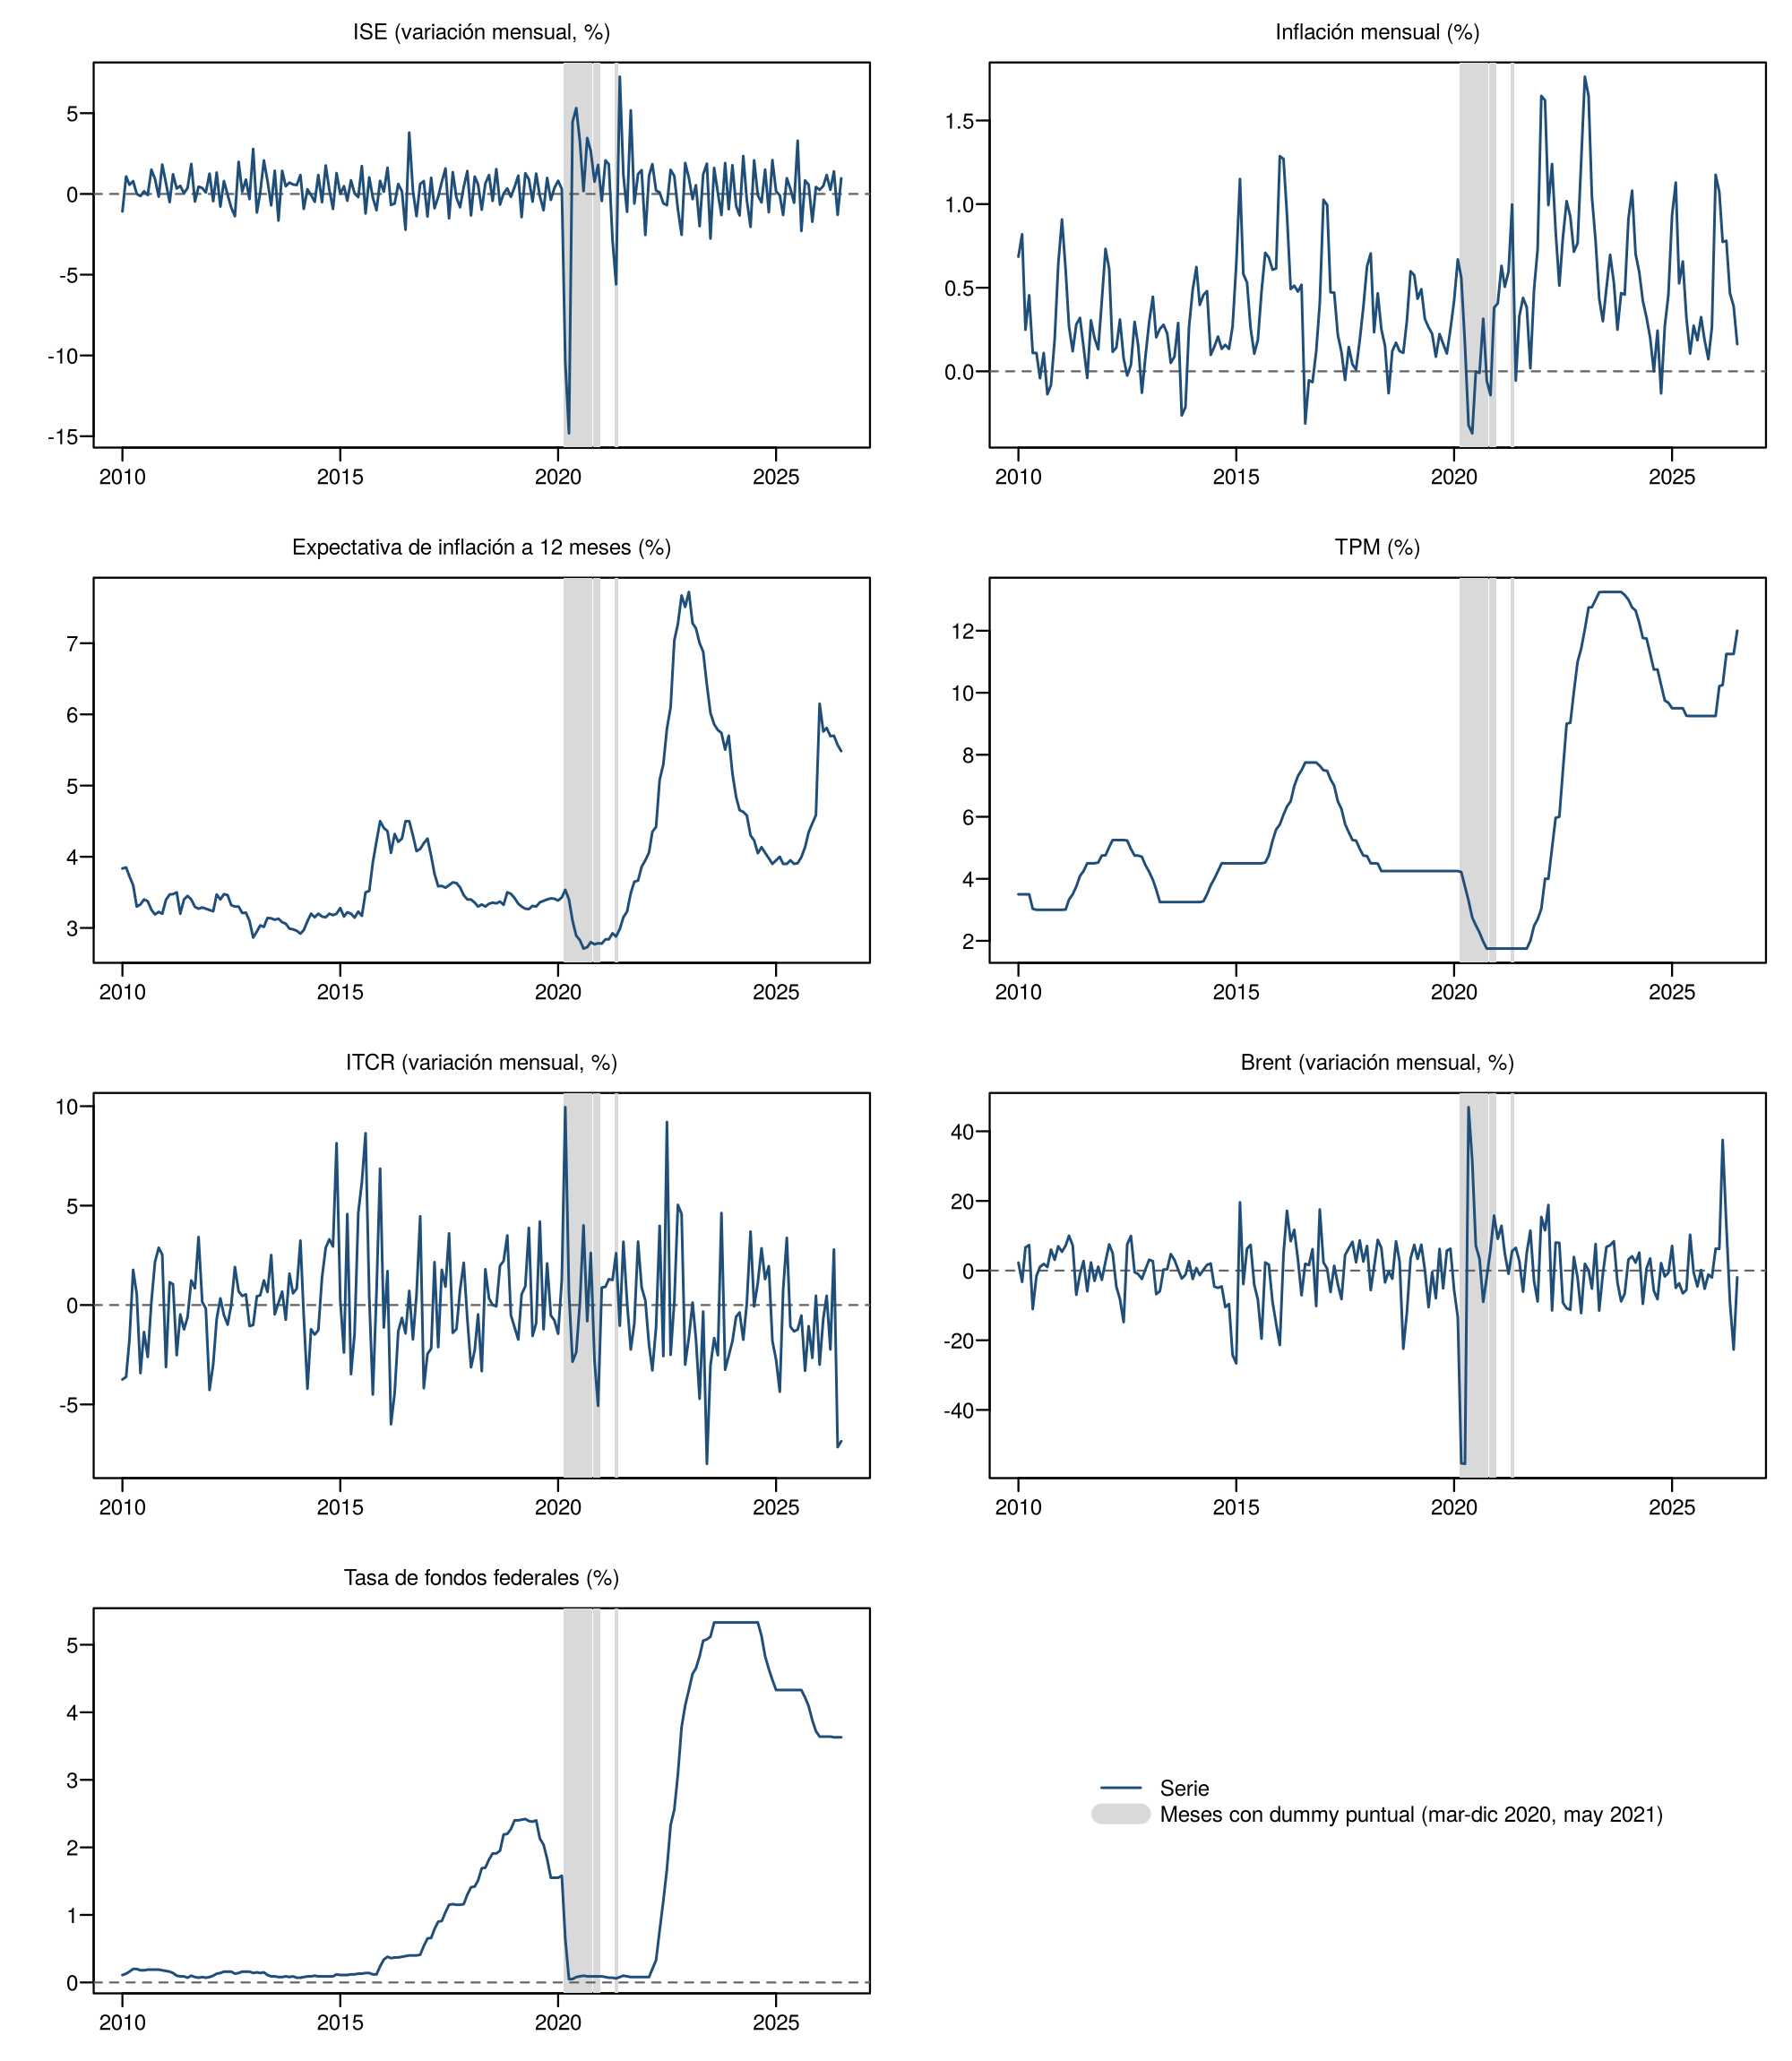
\includegraphics[width=\textwidth]{fig_series_var.png}
\caption{Variables del VAR, 2010m1--2026m7}
\label{fig:series}
\notascuadro{\textit{Nota.} Variables transformadas como entran al VAR. El área gris marca los meses con \textit{dummy} puntual (marzo--diciembre de 2020 y mayo de 2021). 

Fuente: Elaboración propia con datos de DANE, Banco de la República y FRED.}
\end{figure}

La Figura~\ref{fig:series} muestra las series tal como entran al VAR. Las variables en variación mensual (ISE, ITCR y Brent) fluctúan alrededor de un nivel estable, mientras que la TPM, las expectativas de inflación y la tasa de la Fed son más persistentes y reflejan los ciclos de política monetaria del periodo. La inflación mensual presenta además un patrón estacional, que se controla con \textit{dummies} estacionales.

En particular, destacan tres episodios. El primero es la pandemia de 2020, con caídas abruptas en la actividad y en el precio del petróleo. El segundo es el paro nacional de mayo de 2021, un periodo de protestas y bloqueos de vías que interrumpió el transporte y el abastecimiento en el país. Ambos se controlan mediante \textit{dummies} puntuales. El tercero es el aumento de la inflación entre 2021 y 2023, que llevó al Banco de la República a elevar la TPM a su nivel más alto de la muestra.

\paragraph{A.4 Raíz unitaria.}

\cuadro{cuadro_raices}

El Cuadro~\ref{tab:raices} resume las pruebas ADF y KPSS, que tienen hipótesis nulas opuestas, de modo que la evidencia es más clara cuando ambas coinciden. El ISE, el ITCR y el Brent tienen raíz unitaria en nivel y son estacionarios en diferencias, por lo que entran al VAR en variaciones mensuales. 

La inflación mensual es estacionaria una vez que se elimina su patrón estacional. La TPM, las expectativas y la tasa de la Fed son muy persistentes, pero se mantienen en nivel por su interpretación económica.

\paragraph{A.5 Estacionalidad del IPC.} 
El IPC no está desestacionalizado, por lo que la inflación es más alta en enero y febrero y más baja a mitad de año (Figura~\ref{fig:estacionalidad}). Si este patrón se repite de forma estable cada año, basta con incluir una \textit{dummy} por mes; si cambia con el tiempo, lo adecuado es usar la inflación anual (Kilian y Lütkepohl, 2017). Las pruebas OCSB y Canova--Hansen indican que el patrón es estable (Cuadro~\ref{tab:estacional}), por lo que la inflación entra al VAR en variación mensual con 11 \textit{dummies} estacionales.
\cuadro{cuadro_estacional}

\begin{figure}[H]
\centering
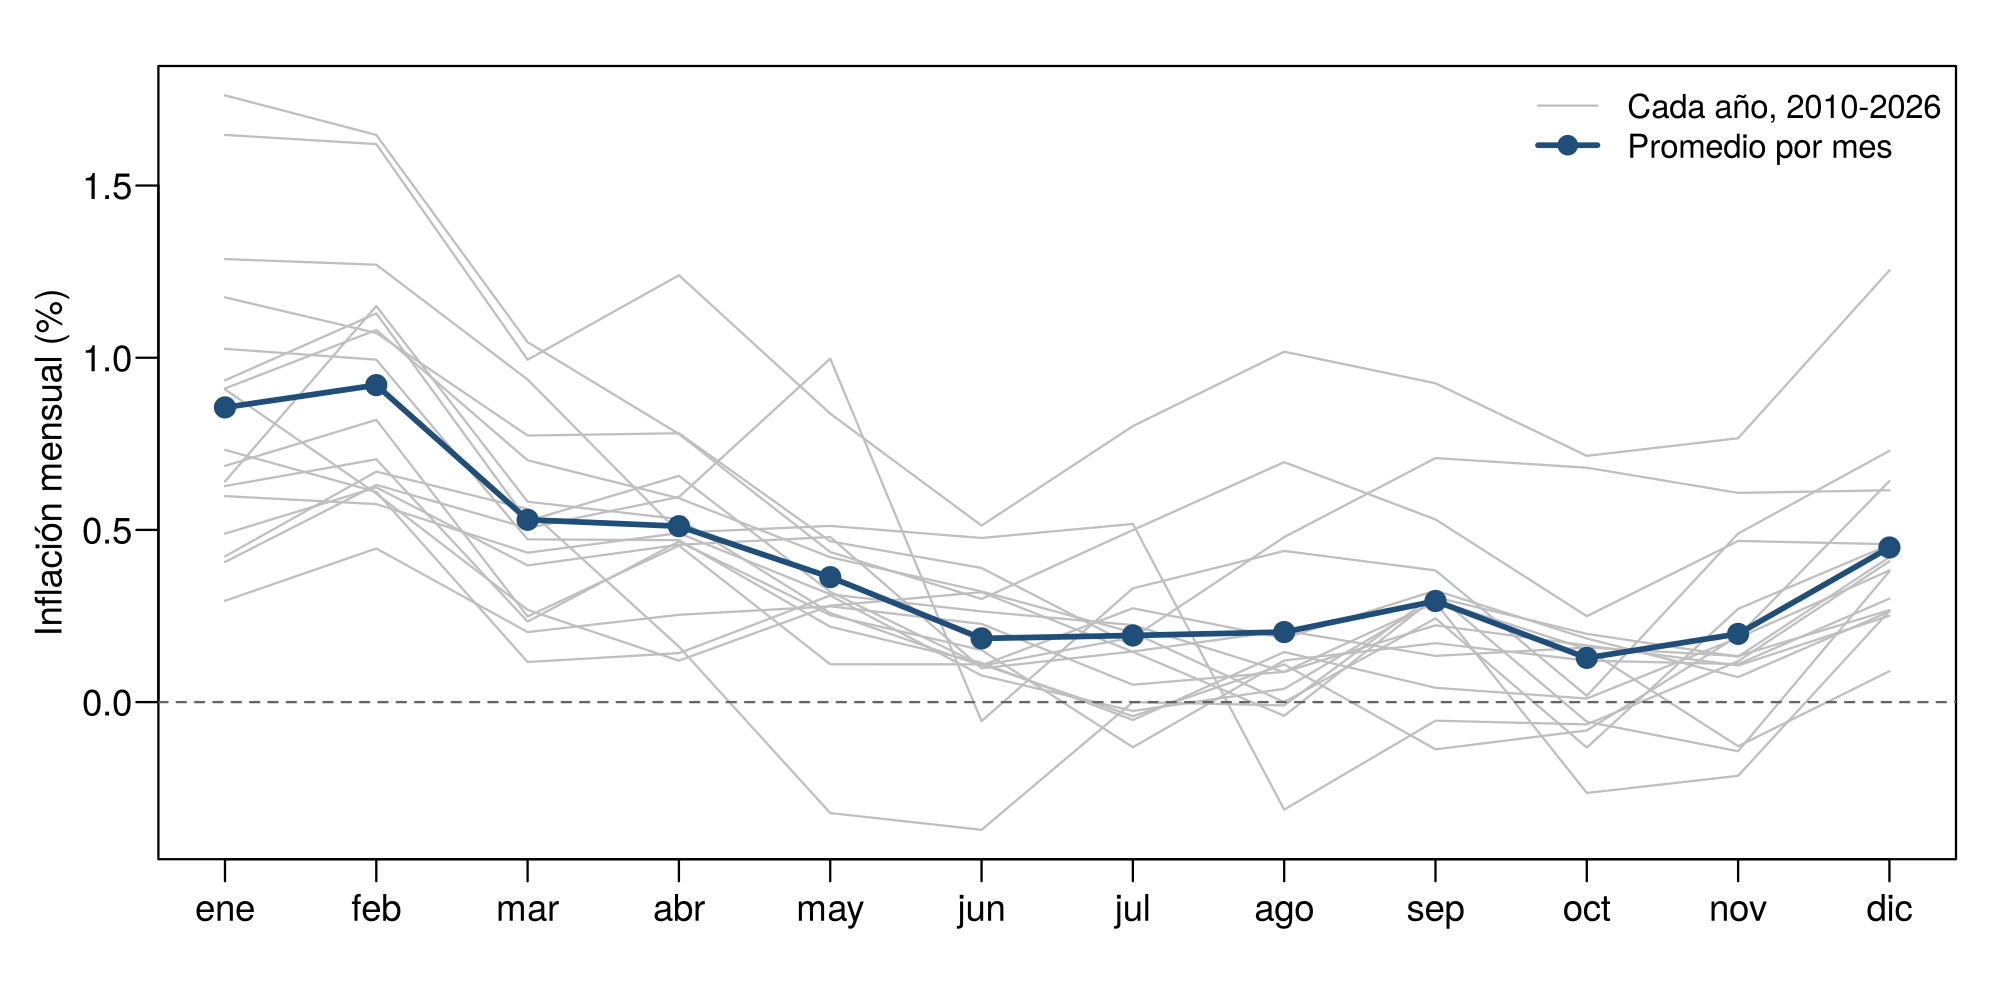
\includegraphics[width=\textwidth]{fig_estacionalidad.png}
\caption{Inflación mensual por mes del año, 2010--2026}
\label{fig:estacionalidad}
\notascuadro{\textit{Nota.} Cada línea gris es un año; la línea azul es el promedio de cada mes. 

Fuente: Elaboración propia con datos de DANE.}
\end{figure}

\paragraph{A.6 Selección de variables y especificaciones alternativas.} El Cuadro~\ref{tab:especificaciones} compara distintas especificaciones del VAR según tres criterios: estabilidad, ausencia de autocorrelación y precisión de los efectos de largo plazo, de los que depende la identificación. Se incluyeron las expectativas de inflación porque permiten evaluar el anclaje de expectativas sin deteriorar el modelo. El crédito real se descartó porque deja autocorrelación en los residuos y, junto con las expectativas, lleva al VAR cerca de la inestabilidad. Las \textit{dummies} puntuales cubren todo 2020, que da mejores diagnósticos que cubrir solo marzo a junio, y mayo de 2021 por el paro nacional.

\cuadro{cuadro_especificaciones}

\cuadro{cuadro_inflacion_anual_mensual}

El Cuadro~\ref{tab:inflacion_anual_mensual} compara el VAR con inflación anual y mensual. Con la inflación anual, el VAR deja de ser estable a partir de 6 rezagos; con la mensual, es estable con cualquier número de rezagos, lo que respalda la elección de la sección anterior.

\subsection*{Anexo B. Identificaci\'on}
\addcontentsline{toc}{subsection}{Anexo B. Identificaci\'on: derivaci\'on}

\paragraph{B.1 Sistema reducido y estructura de las innovaciones.}
El orden de las cinco variables es
\begin{equation}
y_t=\begin{pmatrix}g_t^{ISE}&\pi_t^{m}&\pi_t^{e,12}&i_t&g_t^{ITCR}\end{pmatrix}',
\qquad
\begin{aligned}
g_t^{ISE}&=100\Delta\log ISE_t,\\
\pi_t^{m}&=100\Delta\log IPC_t,\\
g_t^{ITCR}&=100\Delta\log ITCR_t.
\end{aligned}
\label{eq:b_variables}
\end{equation}
La variable $\pi_t^{e,12}$ representa la mediana de la inflación esperada a doce meses e $i_t$ la TPM promedio mensual, ambas sin diferenciar. Un aumento del ITCR representa una depreciación real del peso. La inflación observada se mide mediante la variación logarítmica mensual del IPC, de acuerdo con la especificación utilizada en el VAR reducido.

Con $p=6$ rezagos, el VAR condicionado en variables externas y determinísticas es
\begin{equation}
y_t=c+\sum_{j=1}^{6}A_jy_{t-j}+\Gamma x_t+u_t,
\qquad E(u_tu_t')=\Sigma_u,
\label{eq:b_var}
\end{equation}
donde $x_t$ contiene las transformaciones del Brent, la tasa de la Fed, ambas con un rezago, y las once dummies estacionales y once puntuales descritas en el Anexo~A. Las funciones impulso--respuesta estructurales se calculan manteniendo fija la trayectoria de esas variables.

Se define
\begin{equation}
u_t=H\varepsilon_t,\qquad
E(\varepsilon_t)=0,\qquad E(\varepsilon_t\varepsilon_t')=I_5,
\qquad \Sigma_u=HH'.
\label{eq:b_cov}
\end{equation}
La columna $He_4$ identifica el impacto de la perturbación denominada monetaria, y se elige su orientación para que $h_{44}>0$. En un sistema de cinco variables, $H$ tiene $5^2=25$ elementos, mientras que la matriz simétrica $\Sigma_u$ ofrece $5(5+1)/2=15$ momentos. El número de restricciones independientes requerido \emph{por orden} es, en consecuencia,
\begin{equation}
5^2-\frac{5(5+1)}2=\frac{5(5-1)}2=10.
\label{eq:b_conteo}
\end{equation}

\paragraph{B.2 Las nueve exclusiones contemporáneas.}
Se imponen sobre la matriz de impacto $H$ las igualdades
\begin{align}
h_{12}=h_{13}=h_{14}=h_{15}&=0,\nonumber\\
h_{23}=h_{24}=h_{25}&=0,\nonumber\\
h_{34}=h_{35}&=0.
\label{eq:b_ceros}
\end{align}
La matriz admisible tiene el patrón de la ecuación~\eqref{eq:p1_H}; $h_{45}$ y $h_{54}$ permanecen libres. El Cuadro~\ref{tab:fundamentos_p1} distingue la motivación económica y las limitaciones de cada restricción.

\begingroup
\footnotesize
\setlength{\tabcolsep}{2.5pt}
\renewcommand{\arraystretch}{1.16}

\begin{longtable}{@{}>{\raggedright\arraybackslash}p{0.16\textwidth}>{\raggedright\arraybackslash}p{0.25\textwidth}>{\raggedright\arraybackslash}p{0.30\textwidth}>{\raggedright\arraybackslash}p{0.23\textwidth}@{}}
\caption{Fundamentación teórica y empírica de las restricciones de identificación de la propuesta 1 (P1)}\label{tab:fundamentos_p1}\\
\toprule
\textbf{Restricción} & \textbf{Fundamento teórico} & \textbf{Evidencia empírica} & \textbf{Limitaciones y alcance}\\
\midrule
\endfirsthead

\multicolumn{4}{@{}l}{\textit{Cuadro \thetable\ (continuación)}}\\
\toprule
\textbf{Restricción} & \textbf{Fundamento teórico} & \textbf{Evidencia empírica} & \textbf{Limitaciones y alcance}\\
\midrule
\endhead

\midrule
\multicolumn{4}{r@{}}{\footnotesize\textit{Continúa en la página siguiente}}\\
\endfoot

\bottomrule
\endlastfoot

\textbf{$h_{12}=0$}\newline
Inflación $\rightarrow$ ISE.
& Las decisiones de producción y gasto pueden ajustarse con rezago ante innovaciones de precios, debido a compromisos y costos de ajuste.
& González-Téllez y Laborde-Vera (2026) documentan una transmisión monetaria dinámica y heterogénea sobre actividad y precios en Colombia.
& Las perturbaciones de oferta y costos pueden modificar precios y producción dentro del mismo mes. No existe verificación directa de que el impacto sea exactamente nulo.\\
\midrule

\textbf{$h_{13}=0$}\newline
Expectativas $\rightarrow$ ISE.
& Los cambios de expectativas pueden alterar planes de consumo, inversión y producción, aunque parte de su ejecución toma tiempo.
& Rincón-Torres, Salas-Ávila y Julio-Román (2023) documentan información escalonada, desacuerdos entre agentes y ajustes graduales de expectativas en Colombia.
& Una noticia puede modificar gasto e inversión inmediatamente. La incorporación gradual de información no prueba un cero contemporáneo del ISE.\\
\midrule

\textbf{$h_{14}=0$}\newline
Shock monetario $\rightarrow$ ISE.
& Los canales de tasas, financiamiento y demanda actúan con rezagos, como en modelos de transmisión monetaria con rigideces nominales y reales. Bj{\o}rnland (2009) utiliza exclusiones contemporáneas para variables domésticas.
& González-Téllez y Laborde-Vera (2026) estiman efectos contractivos de sorpresas monetarias sobre la actividad colombiana, con una transmisión dinámica y diferencias regionales.
& Las decisiones financieras y productivas pueden anticiparse o reaccionar dentro del mes; la literatura no establece que el impacto sea exactamente cero.\\
\midrule

\textbf{$h_{15}=0$}\newline
Shock cambiario $\rightarrow$ ISE.
& Los efectos sobre competitividad, costos de importación y balances requieren ajustes de producción y gasto que pueden ser graduales.
& Quintero Otero y Ruíz Celis (2019) documentan respuestas heterogéneas de la producción sectorial colombiana ante movimientos cambiarios.
& Empresas importadoras, exportadoras y endeudadas en divisas pueden reaccionar dentro del mes. La evidencia de efectos sectoriales no valida el cero de impacto agregado.\\
\midrule

\textbf{$h_{23}=0$}\newline
Expectativas $\rightarrow$ inflación mensual.
& La fijación escalonada de precios y los contratos pueden retrasar el traspaso de cambios en expectativas al IPC; sin embargo, la curva de Phillips neokeynesiana incorpora expectativas futuras en la inflación corriente.
& Sánchez-Jabba y Villabón-Hinestroza (2024) encuentran un traspaso importante de expectativas de encuestas a la inflación colombiana; Huertas-Campos y Salazar-Silva (2026) también destacan su relevancia en la inflación de bienes.
& La evidencia favorece la existencia del canal, no su ausencia contemporánea.\\
\midrule

\textbf{$h_{24}=0$}\newline
Shock monetario $\rightarrow$ inflación mensual.
& Las decisiones de tasa se transmiten a costos marginales y demanda mediante rezagos; los precios escalonados distribuyen la respuesta inflacionaria en el tiempo.
& González-Téllez y Laborde-Vera (2026) encuentran respuestas desinflacionarias a perturbaciones contractivas en Colombia, sin proporcionar una prueba directa de ausencia de impacto mensual.
& Precios flexibles, costos financieros y anuncios pueden incidir en el mismo mes. No debe confundirse desinflación rezagada con un cero exacto de impacto.\\
\midrule

\textbf{$h_{25}=0$}\newline
Shock cambiario $\rightarrow$ inflación mensual.
& La depreciación se transmite primero a precios importados e insumos y luego al IPC; contratos, márgenes y costos de distribución pueden retrasar el traspaso.
& Rowland (2004) encuentra traspaso incompleto hacia precios al consumidor. Larrahondo et al. (2025) reportan un efecto contemporáneo sobre inflación al consumidor relativamente pequeño frente al registrado en precios importados y al productor.
& El traspaso inicial puede ser positivo. Además, gran parte de la literatura usa el tipo de cambio nominal y nuestro VAR utiliza la variación del ITCR.\\
\midrule

\textbf{$h_{34}=0$}\newline
Shock monetario $\rightarrow$ expectativas a doce meses.
& Se plantea una exclusión de calendario: la encuesta no puede incorporar decisiones de tasa no anticipadas que ocurren después de su levantamiento.
& Iregui-Bohórquez et al. (2021) describen que la encuesta de expectativas se recoge usualmente entre los días 6 y 14. Osorio-Barreto, Mora y Sierra-Suárez (2025) encuentran que las expectativas colombianas sí responden a movimientos de tasas.
& Algunas decisiones pueden preceder la encuesta; existe anticipación y la TPM se mide como promedio mensual. La información temporal no garantiza el cero en cada observación.\\
\midrule

\textbf{$h_{35}=0$}\newline
Shock cambiario $\rightarrow$ expectativas a doce meses.
& Si una perturbación cambiaria se produce después del levantamiento de la encuesta, no puede modificar retrospectivamente las expectativas ya reportadas.
& Iregui-Bohórquez et al. (2021) documentan el calendario de la encuesta. Osorio-Barreto et al. (2025) encuentran sensibilidad de las expectativas de inflación ante perturbaciones cambiarias.
& El ITCR mensual incorpora información previa y posterior a la encuesta, mientras los agentes observan diariamente el mercado cambiario.\\
\midrule

\textbf{$e_5'A(1)^{-1}He_4=0$}\newline
Neutralidad de largo plazo del ITCR.
& Una perturbación monetaria puede modificar transitoriamente precios relativos mediante rigideces nominales, sin desplazar permanentemente el tipo de cambio real de equilibrio. Utilizada por Bj{\o}rnland (2009).
& Arias y Misas (1998) estudian la neutralidad monetaria del TCR colombiano mediante un SVAR y atribuyen las fluctuaciones permanentes principalmente a perturbaciones reales. Bj{\o}rnland (2009) analiza ajustes cambiarios con neutralidad real a largo plazo.
& Arias y Misas también imponen condiciones de largo plazo. La convergencia de la respuesta acumulada del ITCR a cero se obtiene por construcción.\\
\midrule

\textbf{$h_{45}$ y $h_{54}$ libres}\newline
Simultaneidad TPM--ITCR.
& En economía abierta, la autoridad puede responder a presiones cambiarias y los activos en pesos pueden reaccionar inmediatamente a una sorpresa de tasas. No se impone el signo cambiario.
& Bj{\o}rnland (2009) permite interacción contemporánea entre tasa y tipo de cambio. Echavarría, López-Enciso y Misas (2009) estudian política e intervención cambiaria en Colombia; Gómez-Cardona (2014) analiza respuestas de la autoridad a movimientos cambiarios.
& Dejar ambos coeficientes libres no garantiza distinguir completamente shocks monetarios de perturbaciones de riesgo, financieras o de información.\\
\midrule

\textbf{Brent y Fed exógenos}\newline
Economía pequeña y abierta.
& Se supone que innovaciones exclusivamente colombianas no alteran la tasa de fondos federales ni el precio mundial del petróleo. Sus valores contemporáneos y rezagados condicionan la dinámica doméstica.
& Gómez-Cardona (2014) utiliza una estructura de economía pequeña y abierta para Colombia. González-Téllez y Laborde-Vera (2026) muestran la relevancia de separar sorpresas monetarias de movimientos sistemáticos de la tasa.
& Brent y Fed no agotan la información sobre riesgo soberano, política fiscal, condiciones financieras externas ni intervenciones cambiarias.\\
\midrule

\textbf{Identificación exacta}\newline
Nueve ceros y una neutralidad; $h_{44}>0$.
& Con cinco variables, $H$ tiene 25 coeficientes y $\Sigma_u$ aporta 15 momentos: se requieren diez restricciones de igualdad independientes por orden. El signo $h_{44}>0$ orienta el shock como contractivo; el alza de 25 puntos base es una normalización de escala.
& La estrategia adapta la combinación de restricciones de Bj{\o}rnland (2009). Una rotación ortogonal de las columnas monetaria y cambiaria puede preservar $HH'=\Sigma_u$ y los nueve ceros mientras se impone la neutralidad cambiaria.
& \textbf{Orden no implica automáticamente rango ni causalidad.} Deben verificarse $HH'=\Sigma_u$, los nueve ceros, la neutralidad y la unicidad relevante. La interpretación causal exige supuestos adicionales de exogeneidad e información suficiente.\\
\end{longtable}
\endgroup

\paragraph{B.3 Neutralidad de largo plazo del ITCR.}
Definimos la representación de medias móviles reducida, condicional en las exógenas, como $y_t=\cdots+\sum_{h=0}^{\infty}\Psi_hu_{t-h}$, donde $\Psi_0=I_5$. Las matrices de respuesta estructural son
\begin{equation}
\Theta_h=\Psi_hH,\qquad h=0,1,2,\ldots.
\label{eq:b_irf}
\end{equation}
Si el VAR es estable,
\begin{equation}
A(1)=I_5-\sum_{j=1}^{6}A_j,
\qquad \sum_{h=0}^{\infty}\Psi_h=A(1)^{-1},
\qquad \sum_{h=0}^{\infty}\Theta_h=A(1)^{-1}H.
\label{eq:b_longrun}
\end{equation}
Como la quinta variable es $100\Delta\log ITCR_t$, el efecto de largo plazo sobre el \emph{nivel logarítmico} del ITCR corresponde a la suma de las respuestas de sus variaciones mensuales. La décima restricción de igualdad es
\begin{equation}
\boxed{\ e_5'A(1)^{-1}He_4=\sum_{h=0}^{\infty}e_5'\Theta_he_4=0\ }.
\label{eq:b_nneutralidad}
\end{equation}
La neutralidad de largo plazo se toma de la estrategia de Bj{\o}rnland (2009), adaptada al ITCR colombiano, y es una hipótesis identificadora. No debe describirse como evidencia independiente a favor de la neutralidad a partir de una IRF que converge a cero por construcción.

\paragraph{B.4 Funciones Impulso--Respuesta y normalización.}
Para un choque de una desviación estándar, la respuesta de la variable $j$ en el horizonte $h$ es $e_j'\Psi_hHe_4$. Un aumento de 25 puntos base de la tasa de política monetaria equivale a $0.25$ puntos porcentuales, por lo que, siempre que $h_{44}\ne0$,
\begin{equation}
\operatorname{IRF}_{j}(h;25\,\mathrm{pb})=
\frac{0.25}{h_{44}}e_j'\Psi_hHe_4.
\label{eq:b_norm}
\end{equation}
Para el ISE y el ITCR, sus respuestas de nivel requieren acumular las variaciones mensuales:
\begin{equation}
\operatorname{IRF}^{\mathrm{nivel}}_{j}(h;25\,\mathrm{pb})=
\frac{0.25}{h_{44}}\sum_{s=0}^{h}e_j'\Psi_sHe_4,
\quad j\in\{1,5\}.
\label{eq:b_acum}
\end{equation}
Se interpretan aproximadamente como variaciones porcentuales de los niveles originales, puesto que el VAR modela diferencias logarítmicas multiplicadas por 100. La ecuación~\eqref{eq:b_nneutralidad} garantiza que el efecto acumulado del ITCR converja a cero en el horizonte infinito, pero no impone neutralidad del nivel del ISE.

\paragraph{B.5 Alcance económico e inferencia.}
La estructura permite respuestas contemporáneas mutuas entre TPM e ITCR y no impone el signo del canal cambiario. No obstante, los ceros sobre actividad, inflación mensual y expectativas constituyen restricciones exactas dentro de un mes calendario; las noticias macroeconómicas pueden anticiparse y el Banco de la República puede reaccionar a información no observada por el sistema. El Brent y la tasa de la Fed se incluyen como controles externos, pero ello no asegura que se hayan separado perturbaciones de riesgo, intervenciones cambiarias y cambios en las expectativas sobre la política futura. A su vez, una neutralidad de largo plazo real puede ser discutible si existen fricciones financieras o efectos persistentes sobre la inversión.

Para interpretar la incertidumbre de las funciones impulso--respuesta, cada réplica de remuestreo debe volver a estimar el VAR y recuperar la matriz $H$ bajo las diez restricciones, con la normalización monetaria correspondiente. Los detalles del procedimiento y de las pruebas de robustez pertenecen al Anexo~D. La identificación exacta es una propiedad algebraica \emph{condicionada a los supuestos}, no una demostración de que el shock recuperado sea una innovación monetaria causal y pura.

\subsection*{Anexo C. Estimación}
\addcontentsline{toc}{subsection}{Anexo C. Estimación}

El VAR en forma reducida es
\begin{equation}
y_t = c + \sum_{i=1}^{6} A_i y_{t-i} + \Gamma x_t + u_t, \qquad E[u_t u_t'] = \Sigma_u,
\end{equation}
con $y_t = (\Delta\text{ISE}_t, \pi_t, \pi^e_t, \text{TPM}_t, \Delta\text{ITCR}_t)'$, donde $\pi_t$ es la inflación mensual, y $x_t$ igual al Brent y la tasa de la Fed en $t$ y $t-1$, las 11 \textit{dummies} estacionales y las 11 \textit{dummies} puntuales. Cada ecuación tiene 57 regresores y se estima por MCO con 199 observaciones.

\paragraph{C.1 Selección de rezagos.} El Cuadro~\ref{tab:rezagos} reporta los criterios de información, calculados con la misma muestra para todos los rezagos. El criterio de Akaike elige cinco, el de Hannan--Quinn cuatro y el de Schwarz uno, sin embargo, se usan seis porque, en la estimación de respuestas al impulso, omitir rezagos distorsiona sobre todo los horizontes largos, mientras que incluir uno de más solo reduce algo la precisión (Kilian y Lütkepohl, 2017).

Lo anterior es especialmente relevante porque la restricción de largo plazo depende de la suma de todos los coeficientes del VAR. Las pruebas de razón de verosimilitud indican que el quinto rezago es significativo y que del sexto al octavo no cambian el ajuste de manera significativa.

\cuadro{cuadro_rezagos}

\paragraph{C.2 Diagnósticos.} 
El Cuadro~\ref{tab:diagnosticos} compara los diagnósticos con 4, 5, 6 y 8 rezagos. Podemos observar que con seis, el VAR es estable (raíz más grande de 0.949) y no queda autocorrelación relevante en los residuos. Los residuos del ISE y de la TPM muestran heterocedasticidad condicional, y los del ISE, la inflación y las expectativas no son normales, por lo que los intervalos de confianza se construyen con un método robusto a ambos problemas. Las \textit{dummies} estacionales solo son significativas en la ecuación de inflación, la única serie no desestacionalizada.

\cuadro{cuadro_diagnosticos}

La Figura~\ref{fig:residuos} muestra los residuos de cada ecuación. En general, fluctúan alrededor de cero sin tendencias ni patrones persistentes y se mantienen, en su mayoría, dentro de dos desviaciones estándar, lo que es consistente con la ausencia de autocorrelación. Sin embargo, su variabilidad no es constante: los episodios de mayor volatilidad se concentran después de la pandemia, lo que refleja la heterocedasticidad condicional detectada en las pruebas.

\begin{figure}[H]
\centering
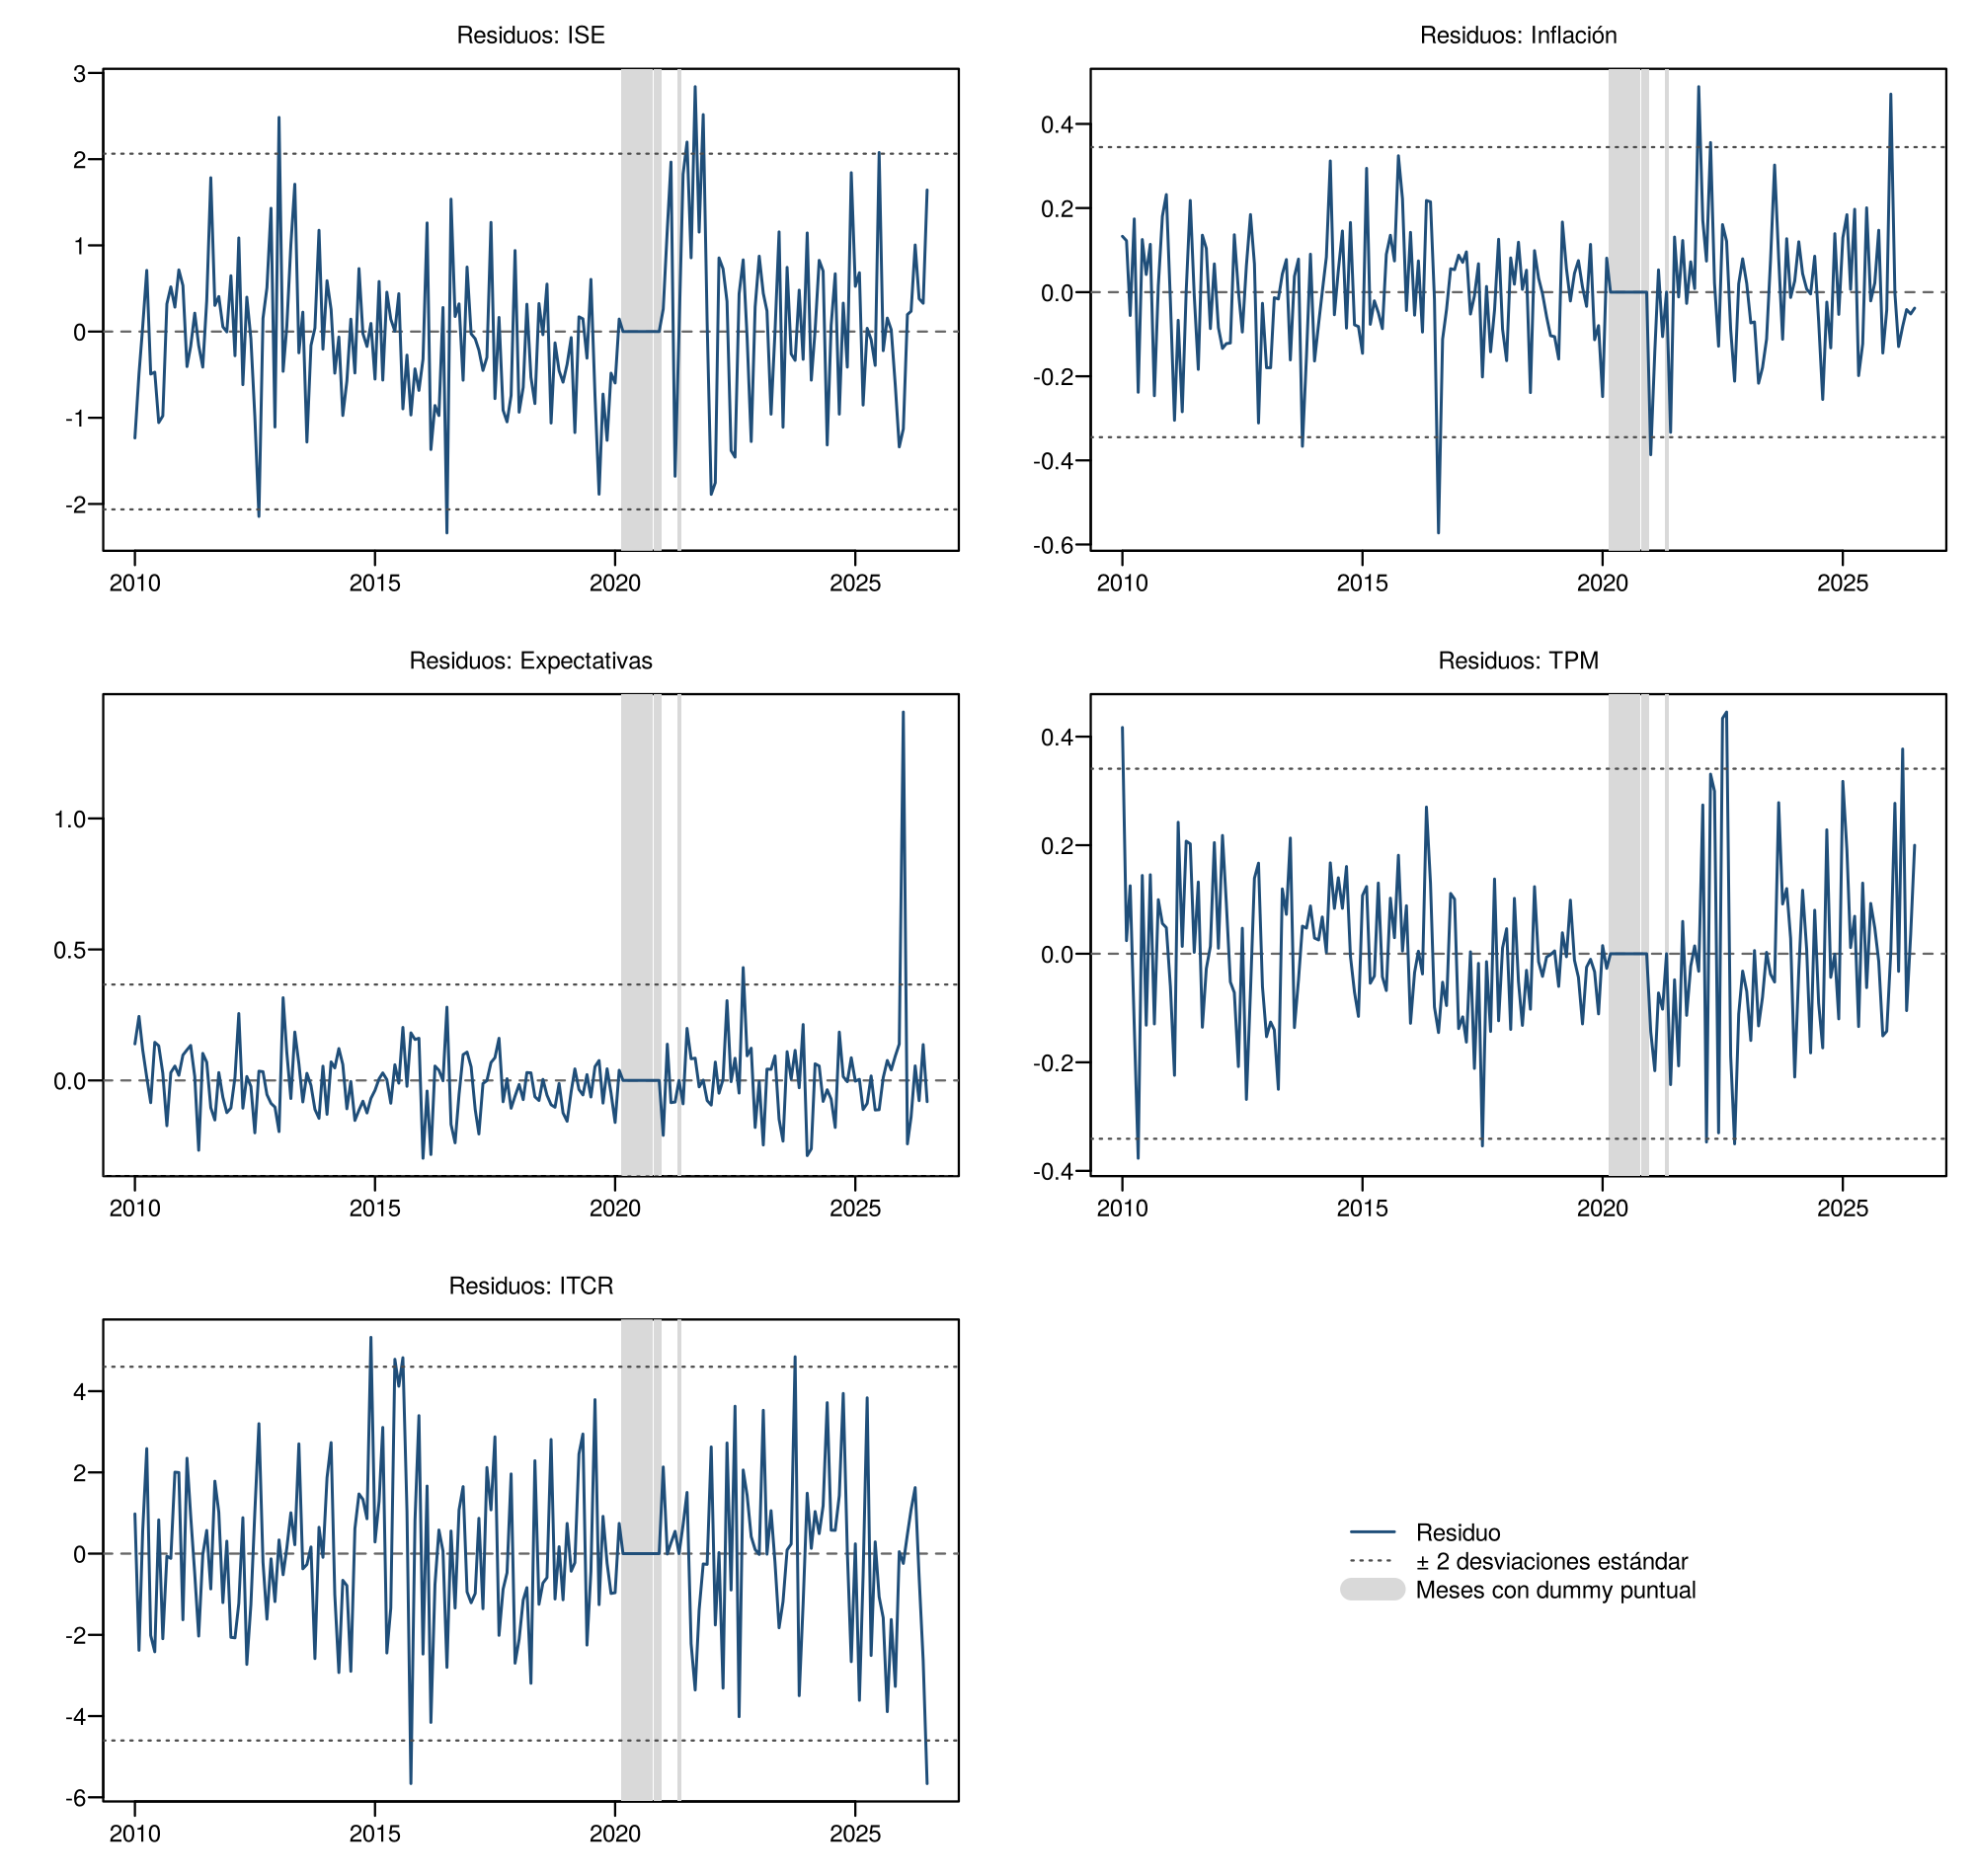
\includegraphics[width=\textwidth]{fig_residuos.png}
\caption{Residuos del VAR con 6 rezagos}
\label{fig:residuos}
\notascuadro{\textit{Nota.} Las líneas punteadas marcan $\pm 2$ desviaciones estándar. El área gris corresponde a los meses con \textit{dummy} puntual, cuyos residuos son cero.

Fuente: Elaboración propia con datos de la DANE y Banco de la República.}
\end{figure}

\paragraph{C.3 Coeficientes estimados.} Los Cuadros~\ref{tab:coeficientes} y~\ref{tab:coeficientes_exogenas} presentan los coeficientes estimados, y el Cuadro~\ref{tab:sigma}, la matriz de covarianzas de los residuos, que es el insumo de la identificación. Los coeficientes individuales de un VAR no tienen una interpretación económica directa; esta se obtiene a partir de las respuestas al impulso.

\cuadro{cuadro_coeficientes}
\cuadro{cuadro_coeficientes_exogenas}
\cuadro{cuadro_sigma}

\paragraph{C.4 De la forma reducida a la matriz de impacto.} Con $\hat A_i$ y $\hat\Sigma_u$, la matriz de impacto $\hat H$, que cumple $\hat H \hat H' = \hat\Sigma_u$ y las restricciones de la sección 3, se calcula en tres pasos:
\begin{enumerate}[leftmargin=1.5em, itemsep=2pt, topsep=4pt]
\item La descomposición de Cholesky de $\hat\Sigma_u$ da una matriz triangular $P$ que ya cumple los nueve ceros de corto plazo.
\item Las dos últimas columnas de $P$, asociadas a la TPM y al ITCR, se rotan un ángulo $\theta$, elegido para que el efecto de largo plazo del choque monetario sobre el nivel del ITCR sea cero. La rotación no altera los ceros del paso anterior ni la igualdad $\hat H \hat H' = \hat\Sigma_u$. El ángulo estimado es de 5.9 grados.
\item Se normaliza el signo para que el choque monetario eleve la TPM en el mes del impacto, y las respuestas se reescalan a un alza de 25 puntos base.
\end{enumerate}
Como hay tantas restricciones como parámetros libres, la solución es única y no requiere métodos numéricos. El Cuadro~\ref{tab:impacto} muestra $\hat H$ y la matriz de efectos de largo plazo, donde se pueden verificar las diez restricciones.

\cuadro{cuadro_impacto}

\subsection*{Anexo D. Inferencia, resultados y robustez}
\addcontentsline{toc}{subsection}{Anexo D. Inferencia, resultados y robustez}

% =============================================================================
\subsubsection*{D.1 Inferencia}

\paragraph{D.1.1 Por qué no el método delta, el bootstrap estándar ni el \textit{wild}.}

\subparagraph{Método delta, bootstrap estándar y \textit{wild bootstrap}.}
Para la inferencia con restricciones de corto o largo plazo, Kilian y Lütkepohl (2017), presentan diversos métodos posibles.
Comienzan presentando entre ellos, el método delta, posteriormente discuten el bootstrap estándar, \textit{wild bootstrap} y el bootstrap por bloques.
De estos métodos de inferencia, el que se ha elegido es el método bootstrap por bloques. Lo cual tiene justificación teórica y empírica, con los datos del ejercicio.

Primero, de manera teórica, se tiene que el método delta asume que los errores del VAR son Gaussianos iid, mientras que los estimadores bootstrap basados en residuos se mantienen válidos asintóticamente aun con condiciones más débiles.

Luego, los métodos bootstrap funcionan a partir de métodos de simulación. Una ventaja es que permiten inferencia en funciones aun cuando las soluciones de forma cerrada del estimador de la varianza no están disponibles o son inconvenientes.

Nótese que en estos casos $g$ no es tan lineal (hay una matriz inversa, arcotangente, cociente). La muestra es corta.

Además, los intervalos de confianza a través de bootstrap tienden a ser más precisos en muestras pequeñas que las aproximaciones asintóticas, y pueden mejorar la precisión de la aproximación asintótica.

Sin embargo, dentro de los métodos de bootstrap, el estándar no es el más conveniente, ya que requiere que el error de regresión sea iid. Lo cual es un supuesto fuerte. Una aproximación alternativa es el \textit{wild bootstrap}, el cual se usó inicialmente para regresiones con heterocedasticidad incondicional.

Sin embargo, se ha mostrado que este método subestima la varianza asintótica de la varianza del error. Produce intervalos de confianza que son muy estrechos y tiene una precisión de cobertura que es muy baja asintóticamente.

Brüggemann, Jentsch y Trenkler (2016) proponen un método bootstrap alternativo, con la intención de asegurar una cobertura asintótica amplia para impulsos respuesta estructurales en cada horizonte: métodos \textit{bootstrap} por bloques.

Así mismo, actualmente, se considera que el método bootstrap por bloques es aquél con mayor cobertura cuando se presenta heterocedasticidad condicional en los errores.

Con los datos del modelo, la prueba Jarque-Bera con 6 rezagos rechaza normalidad de los residuos del ISE, inflación y expectativas. De modo que el método de inferencia más acorde a los datos es el bootstrap por bloques.

\Needspace*{8\baselineskip}% que el título no quede solo al pie de la página
\paragraph{D.1.2 Por qué el bootstrap por bloques.}

\subparagraph{Heterocedasticidad condicional en los residuos.}

La siguiente figura muestra los residuos al cuadrado de la forma reducida, divididos entre su promedio. La línea punteada en 1 es la varianza promedio y la línea azul, un promedio móvil de 12 meses. Con varianza constante, la media móvil debería estar constantemente cerca de 1, sin embargo, en la TPM y en el ISE, no ocurre esto, lo cual es síntoma de heterocedasticidad condicional.

Al realizar la prueba ARCH-LM (Engle, 1982), el Cuadro~\ref{tab:D_arch} muestra que se rechaza varianza constante en la ecuación del ISE y de la TPM.

% figura de prog/07_inferencia_P1.R
\begin{figure}[H]
\centering
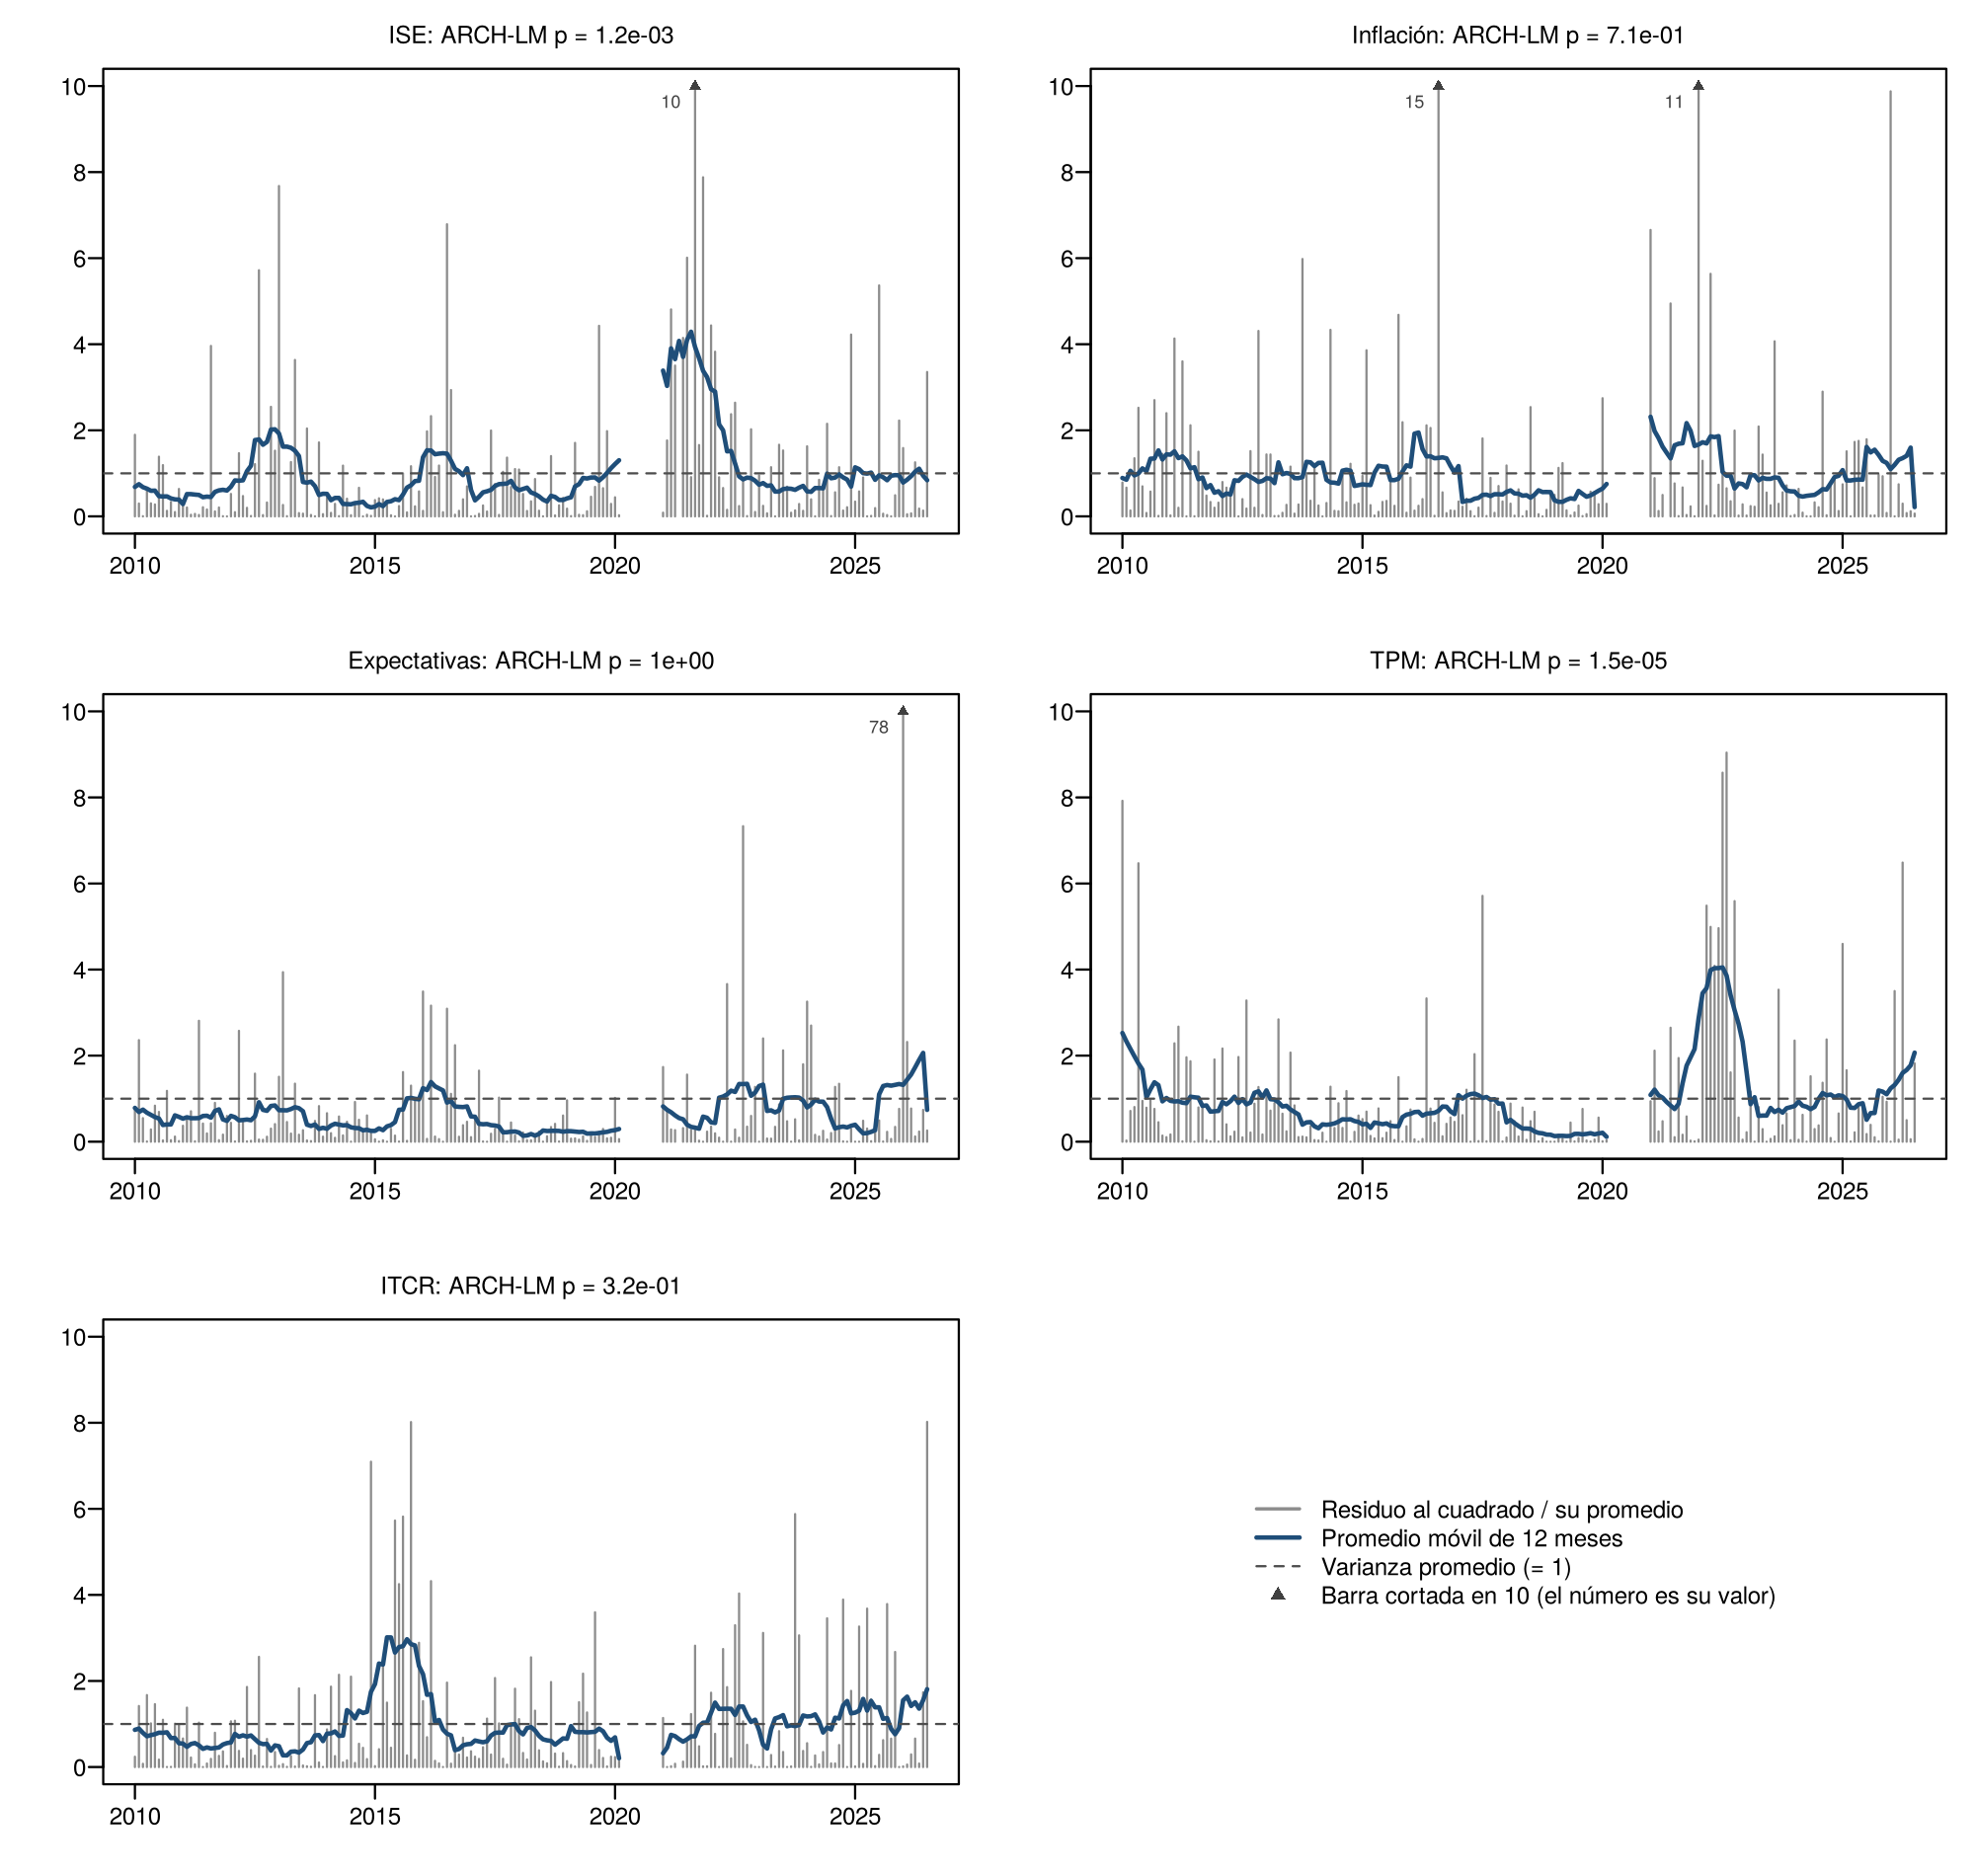
\includegraphics[width=0.85\textwidth]{P1_residuos_ARCH.png}
\caption{Residuos al cuadrado de la forma reducida}
\label{fig:D_residuos_arch}
\notascuadro{\textit{Nota.} En múltiplos de su promedio. El título de cada panel da el valor $p$ de la prueba ARCH-LM.

Fuente: Elaboración propia con datos de DANE y Banco de la República.}
\end{figure}

\cuadro{cuadro_D_arch}

\subparagraph{Algoritmo y cálculo de las bandas.}
\textbf{Definición de banda.} Sea $r_{k,h}$ la respuesta de la variable $k$ en el mes $h$. Una banda de nivel $1-\gamma$ es un intervalo $[\,l_{k,h},\ u_{k,h}\,]$ tal que, si se obtuvieran muchas muestras del mismo proceso y para cada una se calculara la banda con el mismo procedimiento, entonces
\begin{equation}\label{eq:D_cobertura}
P\left(l_{k,h} \le r_{k,h} \le u_{k,h}\right) = 1-\gamma .
\end{equation}
Esa probabilidad se llama \textit{cobertura}.

Para la inferencia del modelo, se usaron $T=199$ meses, $p=6$ rezagos, bloques de $l=12$ meses, y $R=2{,}000$ réplicas.

Algoritmo:

\textbf{Paso 0:} Preparación fuera del bucle (una vez con los datos originales).

(i) Estimación del VAR con los datos originales:
$$y_t = \hat{\nu} + \sum_{j=1}^6 \hat{A}_j y_{t-j} + \hat{\Gamma} x_t + \hat{u}_t, \qquad t = 1, \dots, 199$$

Se guardan las matrices de coeficientes fijos $(\hat{\nu}, \hat{A}_1, \dots, \hat{A}_6, \hat{\Gamma})$ y los $T = 199$ vectores de residuos $\hat{u}_1, \dots, \hat{u}_{199}$.

(ii) Se arma una urna de bloques traslapados y se calculan los promedios de recentrado.

Para no destruir los episodios de volatilidad, se arman bloques móviles traslapados de longitud $l=12$ meses consecutivos.

Son $T-l+1 = 188$ bloques posibles.

$$\begin{aligned} B_1 &= (\hat{u}_1, \hat{u}_2, \dots, \hat{u}_{12}) \\ B_2 &= (\hat{u}_2, \hat{u}_3, \dots, \hat{u}_{13}) \\ &\;\;\vdots \\ B_{188} &= (\hat{u}_{188}, \hat{u}_{189}, \dots, \hat{u}_{199}) \end{aligned}$$

\textbf{Paso 1:} Bloque de simulación, se repite en cada réplica $r=1, \dots, R=2{,}000$.

(i) Como se necesitan cubrir 199 meses con bloques de 12 meses, se necesitan, redondeando hacia arriba, $s = T/l = 199/12 = 16.58$, entonces, 17 bloques.

Luego, se sacan al azar con reemplazo, 17 bloques de la urna de 188, y se apilan uno tras otro en fila.

(ii) Luego, se recentra posición por posición. A cada bloque sorteado, de los $m \in \{1, \dots, 17\}$, en cada vector, de los $i \in \{1, \dots, 12\}$, se le resta el promedio de todos los residuos que pueden caer en esa posición.
$$u_{(m-1)l+i}^* \leftarrow u_{(m-1)l+i}^* - \frac{1}{T - l + 1} \sum_{r=0}^{T-l} \hat{u}_{i+r}, \qquad i = 1, \dots, l$$

(iii) Luego, se mantienen solo las primeras $T=199$ observaciones recentradas, se descartan las 5 sobrantes.

(iv) Posteriormente, se construye una serie artificial de forma recursiva ($y_1^*, \dots, y_T^*$).

Se fijan 6 meses iniciales anteriores a la muestra iguales a los datos reales, es decir, ($y_{-5}^* = y_{-5}, \dots, y_0^* = y_0$), y se dejan fijas las variables exógenas.

Luego, mes a mes, se construye la muestra artificial, metiendo los $y^*$ anteriores como regresores.
Es decir,

$$y_t^* = \hat{\nu} + \sum_{j=1}^6 \hat{A}_j y_{t-j}^* + \hat{\Gamma} x_t + u_t^*, \qquad t = 1, \dots, 199$$

(v) Con la muestra artificial $(y_1^*, \dots, y_{199}^*)$ se estima de nuevo con MCO y se obtienen las matrices estimadas de la réplica: $(\hat{A}_1^*, \dots, \hat{A}_6^*, \hat{\Sigma}^*)$.

Se calculan los valores propios de $\hat{A}^*$, si el módulo de la raíz más grande es mayor o igual que uno, se descarta esa réplica.

(vi) Se reidentifica el choque estructural adentro de la réplica.

\textbf{Paso 2:} Construcción del intervalo.

Sigue tomar percentiles de Efron: Para cada variable $k$, y cada horizonte $h$, se tienen los 2,000 valores simulados $\{\hat{r}_{k,h}^{*(1)}, \dots, \hat{r}_{k,h}^{*(2000)}\}$.

Se ordenan de menor a mayor, y para construir:

Banda de 68\%: se toman los percentiles 16 y 84 de la muestra ordenada.

Banda de 90\%: se toman los percentiles 5 y 95 de la muestra ordenada.

\subparagraph{Bandas de 68\%.}

Por Leamer (1978), y Sims (1987), no hay un estándar universalmente válido para la significancia estadística.

La elección convencional del 5\% de nivel de significancia, es solo una convención que facilita la comunicación para DSEMs muy restringidos, Kilian y Lütkepohl (2017), mencionan que los intervalos de confianza de 68\% (que corresponden a bandas de un error estándar), son más usados al reportar estimaciones para impulsos respuesta estructurales.


\paragraph{D.1.3 Respuestas al impulso con bandas por bloques.}

Los resultados esperados dentro de un marco neokeynesiano (Bj{\o}rnland, 2008) son que, dado un choque contractivo de política monetaria, se espera una reducción en la actividad real, y en la inflación. Además de una apreciación del tipo de cambio.
A su vez, Bj{\o}rnland (2008) encuentra que, en el caso de Noruega, ante un choque contractivo de política monetaria el tipo de cambio real se aprecia gradualmente, que la actividad real se contrae de forma gradual y estadísticamente significativa, y que la inflación anual baja y toca el punto más bajo después de 2.5 años (30 meses).

Luego, en la Figura~\ref{fig:D_irf_bloques}, se presentan las respuestas a un alza de 25 pb en la TPM, con las bandas construidas mediante bootstrap por bloques, con una banda de 68\% y de 90\%.

Hay que notar que, analizando la banda de 68\%, el ISE excluye el cero a partir del mes 5. La inflación anual, muestra una caída significativa a partir del mes 21 hasta el 28. Las expectativas, muestran un alza significativa en el mes 1 y una caída en los meses 20 a 28. El ITCR, muestra una caída desde el mes 13 hasta el 22.

Entonces, los resultados coinciden con Bj{\o}rnland (2008) y con el marco teórico neokeynesiano. El ISE muestra una caída significativa, al igual que la inflación anual, y el ITCR. No hay señales de \textit{price puzzles}, y si bien, las expectativas muestran un alza significativa, es únicamente en el primer mes, posteriormente caen.

% figura de prog/13_cuadros_anexo_D.R, con las bandas de prog/07_inferencia_P1.R
\begin{figure}[H]
\centering
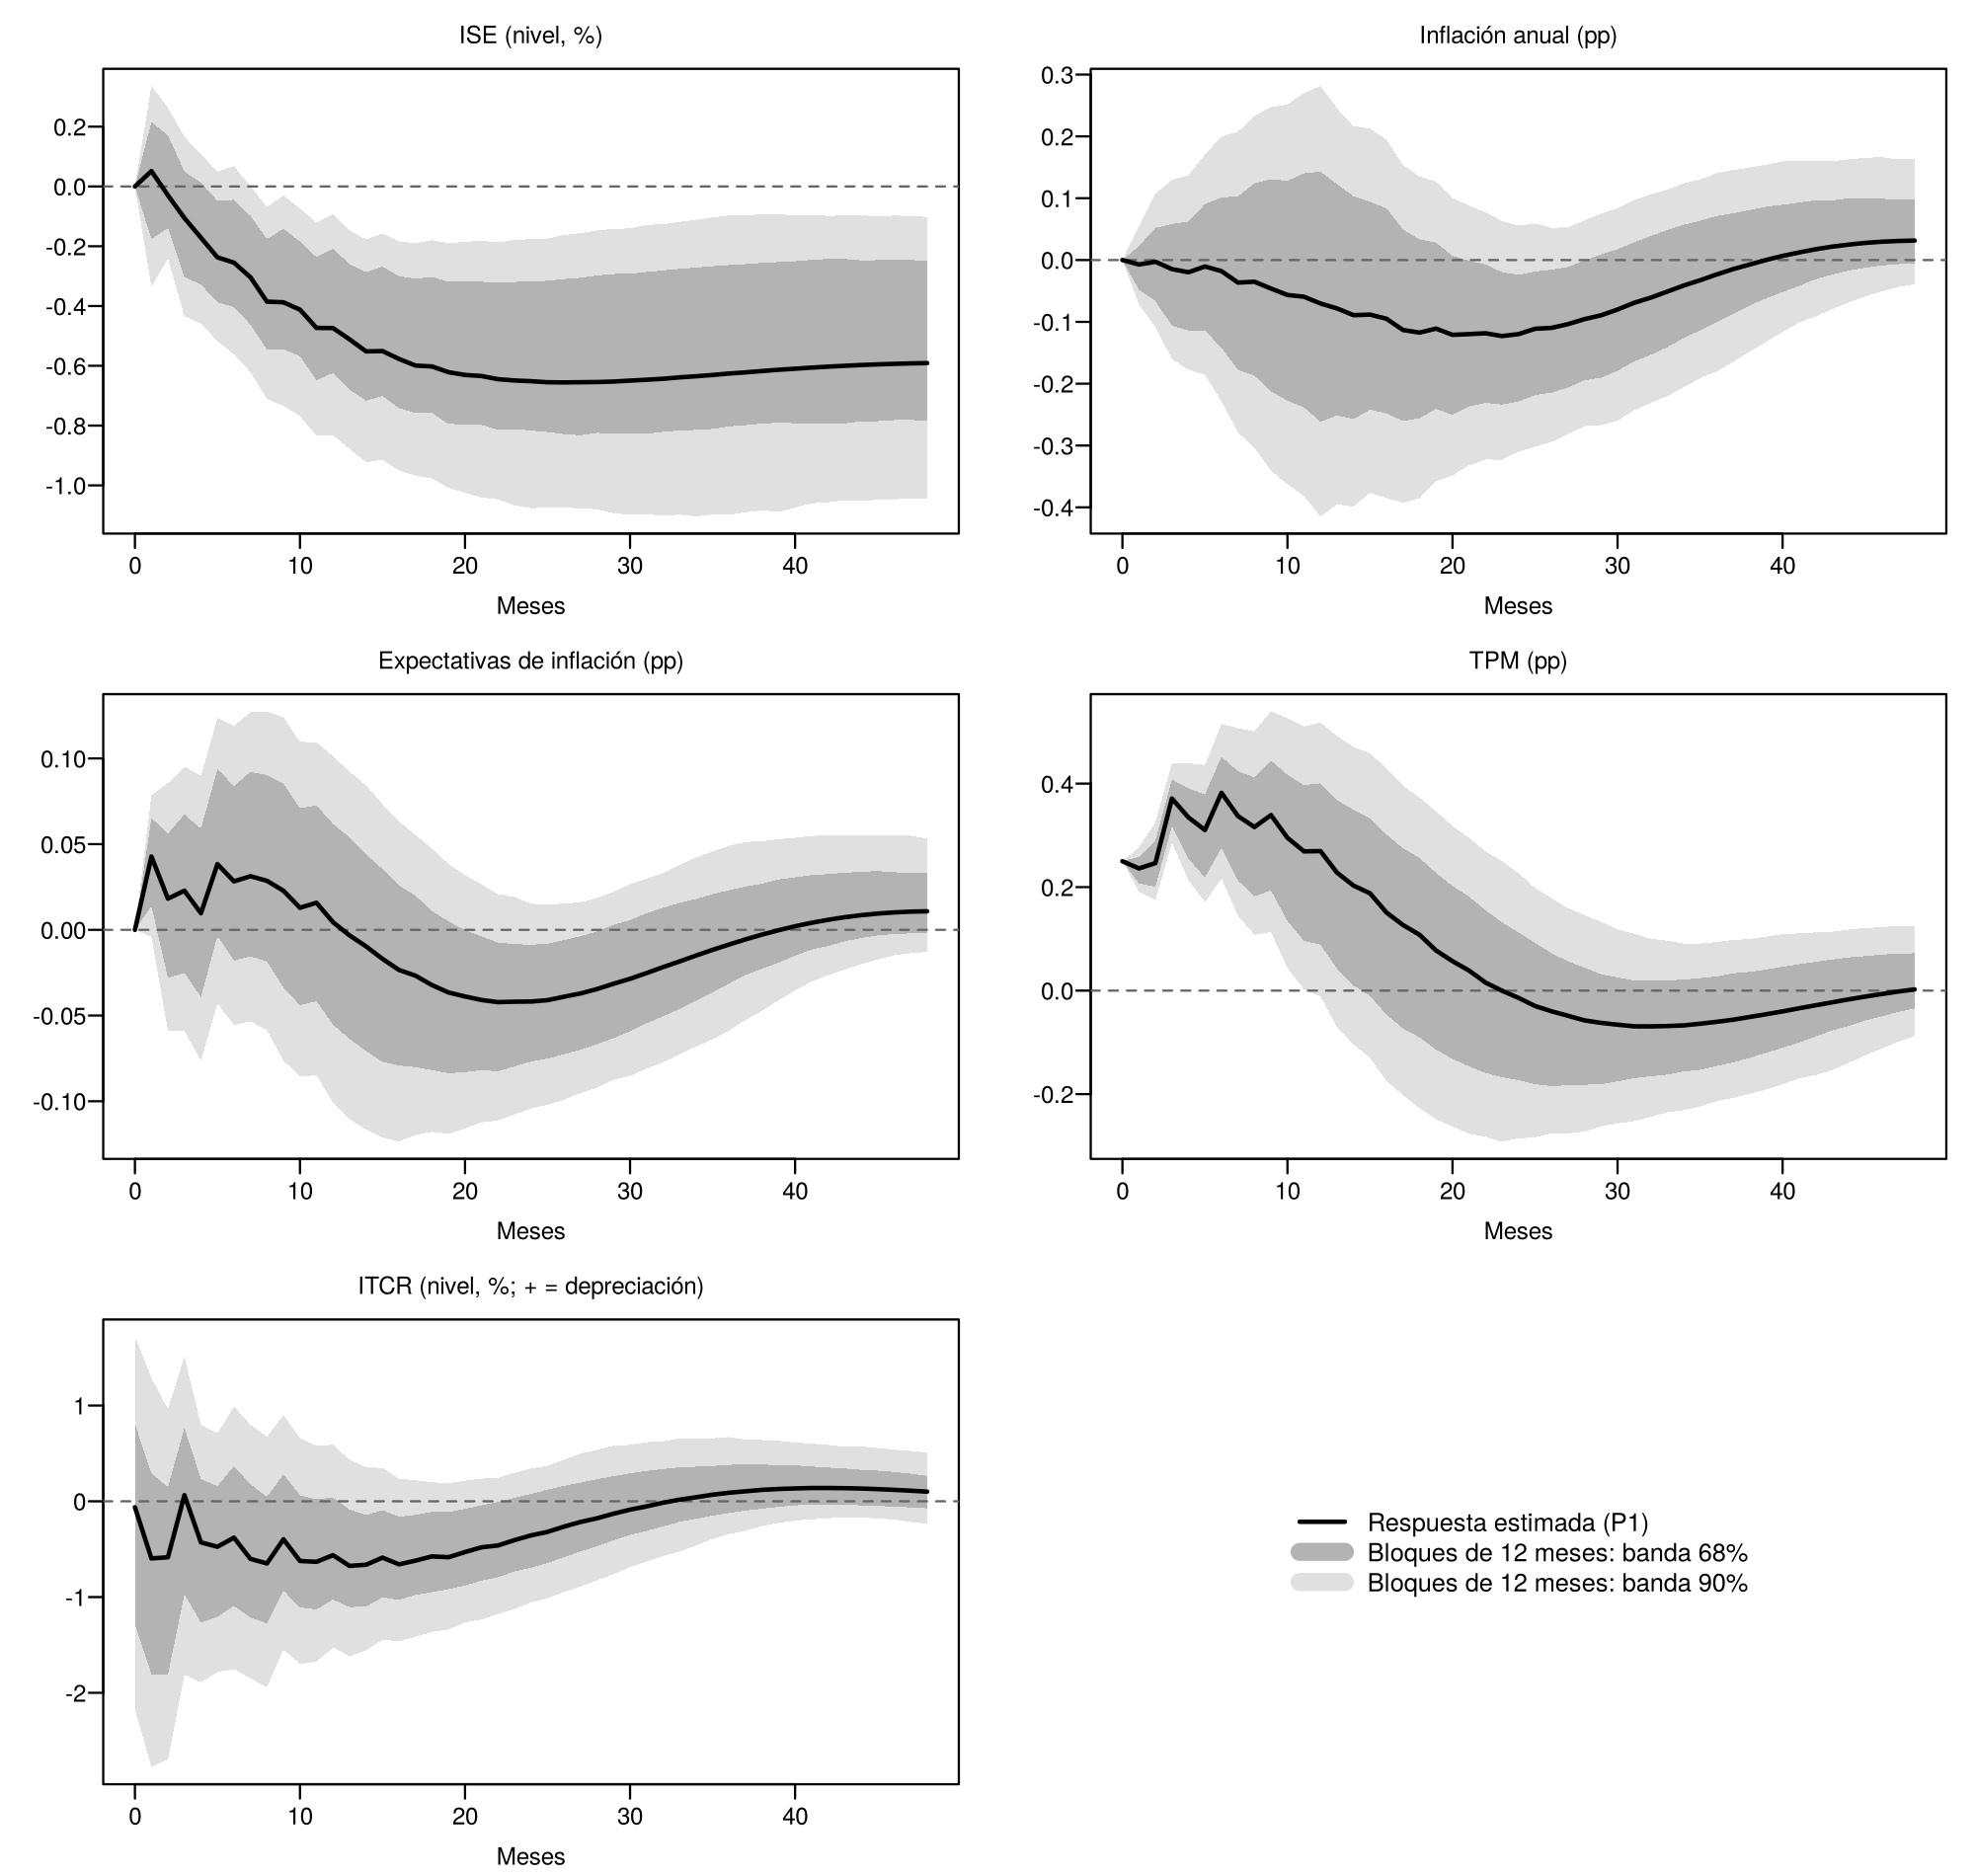
\includegraphics[width=0.85\textwidth]{irf_P1_bloques_solo_25pb.png}
\caption{Respuestas a un alza de 25 pb en la TPM: bootstrap por bloques}
\label{fig:D_irf_bloques}
\notascuadro{\textit{Nota.} 2,000 réplicas por bloques de 12 meses.

Fuente: Elaboración propia con datos de DANE y Banco de la República.}
\end{figure}

A su vez, en el Cuadro~\ref{tab:D_bandas_bloques} se puede observar la estimación por MCO en distintos meses y las bandas de 68\% en bloques de 12 meses y de 24 meses para comparación.

Tanto el ITCR, Inflación y el ISE muestran los signos esperados. Bj{\o}rnland (2008) señala que ante un alza de tasa de interés, se espera una reducción inmediata en el tipo de cambio real, lo cual ocurre en la estimación puntual (aunque no es estadísticamente significativa). La significancia de la caída aparece posteriormente, lo cual se explica ya que, según Bj{\o}rnland (2008), la caída del tipo de cambio real puede aparecer retrasada, aunque Bj{\o}rnland (2008) advierte que el retraso puede venir del orden recursivo de las variables en el VAR.

\cuadro{cuadro_D_bandas_bloques}

Los resultados tienen sentido económico, y son consistentes con la evidencia empírica.

Ante un alza de la TPM, es esperada una entrada de capitales, lo cual provoca una apreciación en el ITCR.

A su vez, tiene sentido que el ISE caiga debido a la reducción en la inversión. También, está bien documentada la caída de la inflación anual ante el alza de la tasa de interés.

% =============================================================================
\subsubsection*{D.2 Resultados generales}

\cuadro{cuadro_D_resultados_generales}

En cuanto a resultados generales, se observa que el ISE alcanza su mínimo alrededor del mes 24 (el mínimo es $-0.66$\% en el mes 26), la inflación anual, de igual manera, alcanza su mínimo en el mes 23 con $-0.12$ pp.

Las expectativas alcanzan un máximo de 0.04 pp, para comenzar a bajar posteriormente, alcanzando el mínimo de $-0.04$ pp en el mes 22.

La TPM alcanza un máximo de 0.38 pp en el mes 6, para caer, y comenzar a ser negativa en el mes 23.

El ITCR, llega a $-0.06$\% en el impacto, con un mínimo de $-0.67$\% en el mes 13, es positivo a partir del mes 33, y dada la restricción, en el largo plazo, llega a 0.

Estos fenómenos tienen sentido según la teoría económica, por ejemplo, el movimiento de la TPM es explicado por el \textit{interest-rate smoothing} (Clarida, Galí y Gertler, 2000), al ver que la tasa no regresa de inmediato a cero después del choque de 0.25 pp. Los bancos centrales suelen implementar los apretones con ciclos graduales y persistentes. Además, la caída posterior muestra la reversión endógena por la regla de Taylor, una vez que el choque deprime el producto, la regla del banco recorta la tasa para estabilizar la economía.

A su vez, Woodford (2003), documenta que la política monetaria impacta plenamente sobre las variables reales a medida que se ajusta la inversión y el consumo, por lo que el horizonte de máxima contracción (24 a 26 meses) es lógico, además de que coincide con Bj{\o}rnland (2008), donde la actividad alcanza su máxima contracción entre 1.5 y 2 años después del choque monetario.

Así mismo, se puede observar que el ISE queda en niveles bajos, lo cual puede explicarse por un efecto de histéresis monetaria, que si bien, en este caso es explicado porque el ISE está en diferencias, y la suma de los efectos puntuales, converge a un número negativo, aunque los efectos en horizontes amplios, sean cero, está documentado que los choques monetarios pueden provocar una contracción real persistente. Laborde-Vera (2026), citando a Jordà et al. (2024), documenta una caída persistente en la actividad a partir de un apretón monetario en EE.UU. en Colombia. La contracción de la actividad real dura hasta 8 años por un efecto duradero sobre la acumulación de capital y la PTF.

El ITCR muestra un comportamiento muy similar al resultado que obtiene Bj{\o}rnland (2008), donde el tipo de cambio real se aprecia durante más de un año, para luego regresar a 0.

Con respecto a la inflación anual, no se logra observar un \textit{price puzzle}, y la secuencia del movimiento está explicada teóricamente (Svensson, 2000). En los modelos neokeynesianos, la política monetaria se transmite hacia la inflación primero, por el canal cambiario (se aprecia el ITCR), y luego por la brecha del producto (ISE, que se profundiza en meses 12 a 26), lo cual es mostrado por los resultados obtenidos en el modelo. La inflación y las expectativas alcanzan sus mínimos en los meses 22 y 23, después del año de apreciación y la contracción de la demanda agregada. Lo cual también coincide con Bj{\o}rnland (2008), donde el punto más bajo de la inflación está alrededor de los 30 meses, y el máximo del desempleo en los 18 meses.

% =============================================================================
\subsubsection*{D.3 Robustez}

\paragraph{D.3.1 Menos y más rezagos.}

En la siguiente gráfica, se muestran ejercicios de robustez, donde se realizó la estimación con 4 y 8 rezagos en lugar de 6.

Los resultados son similares para el ISE con ambas especificaciones.

Con 8 rezagos los resultados se sostienen, con caídas más pronunciadas en el ITCR, inflación, y en las expectativas.

Con 4 rezagos, surge el \textit{price puzzle} en la inflación anual, las expectativas de inflación suben de manera más considerable y la caída del ISE es ligeramente menor. Este \textit{price puzzle} no es significativo: la banda de 68\% nunca queda por encima del cero, y en su punto más alto, $+0.13$ pp en el mes 12, la banda es $[-0.06,\ 0.29]$.

% figura de prog/10_robustez_rezagos.R
\begin{figure}[H]
\centering
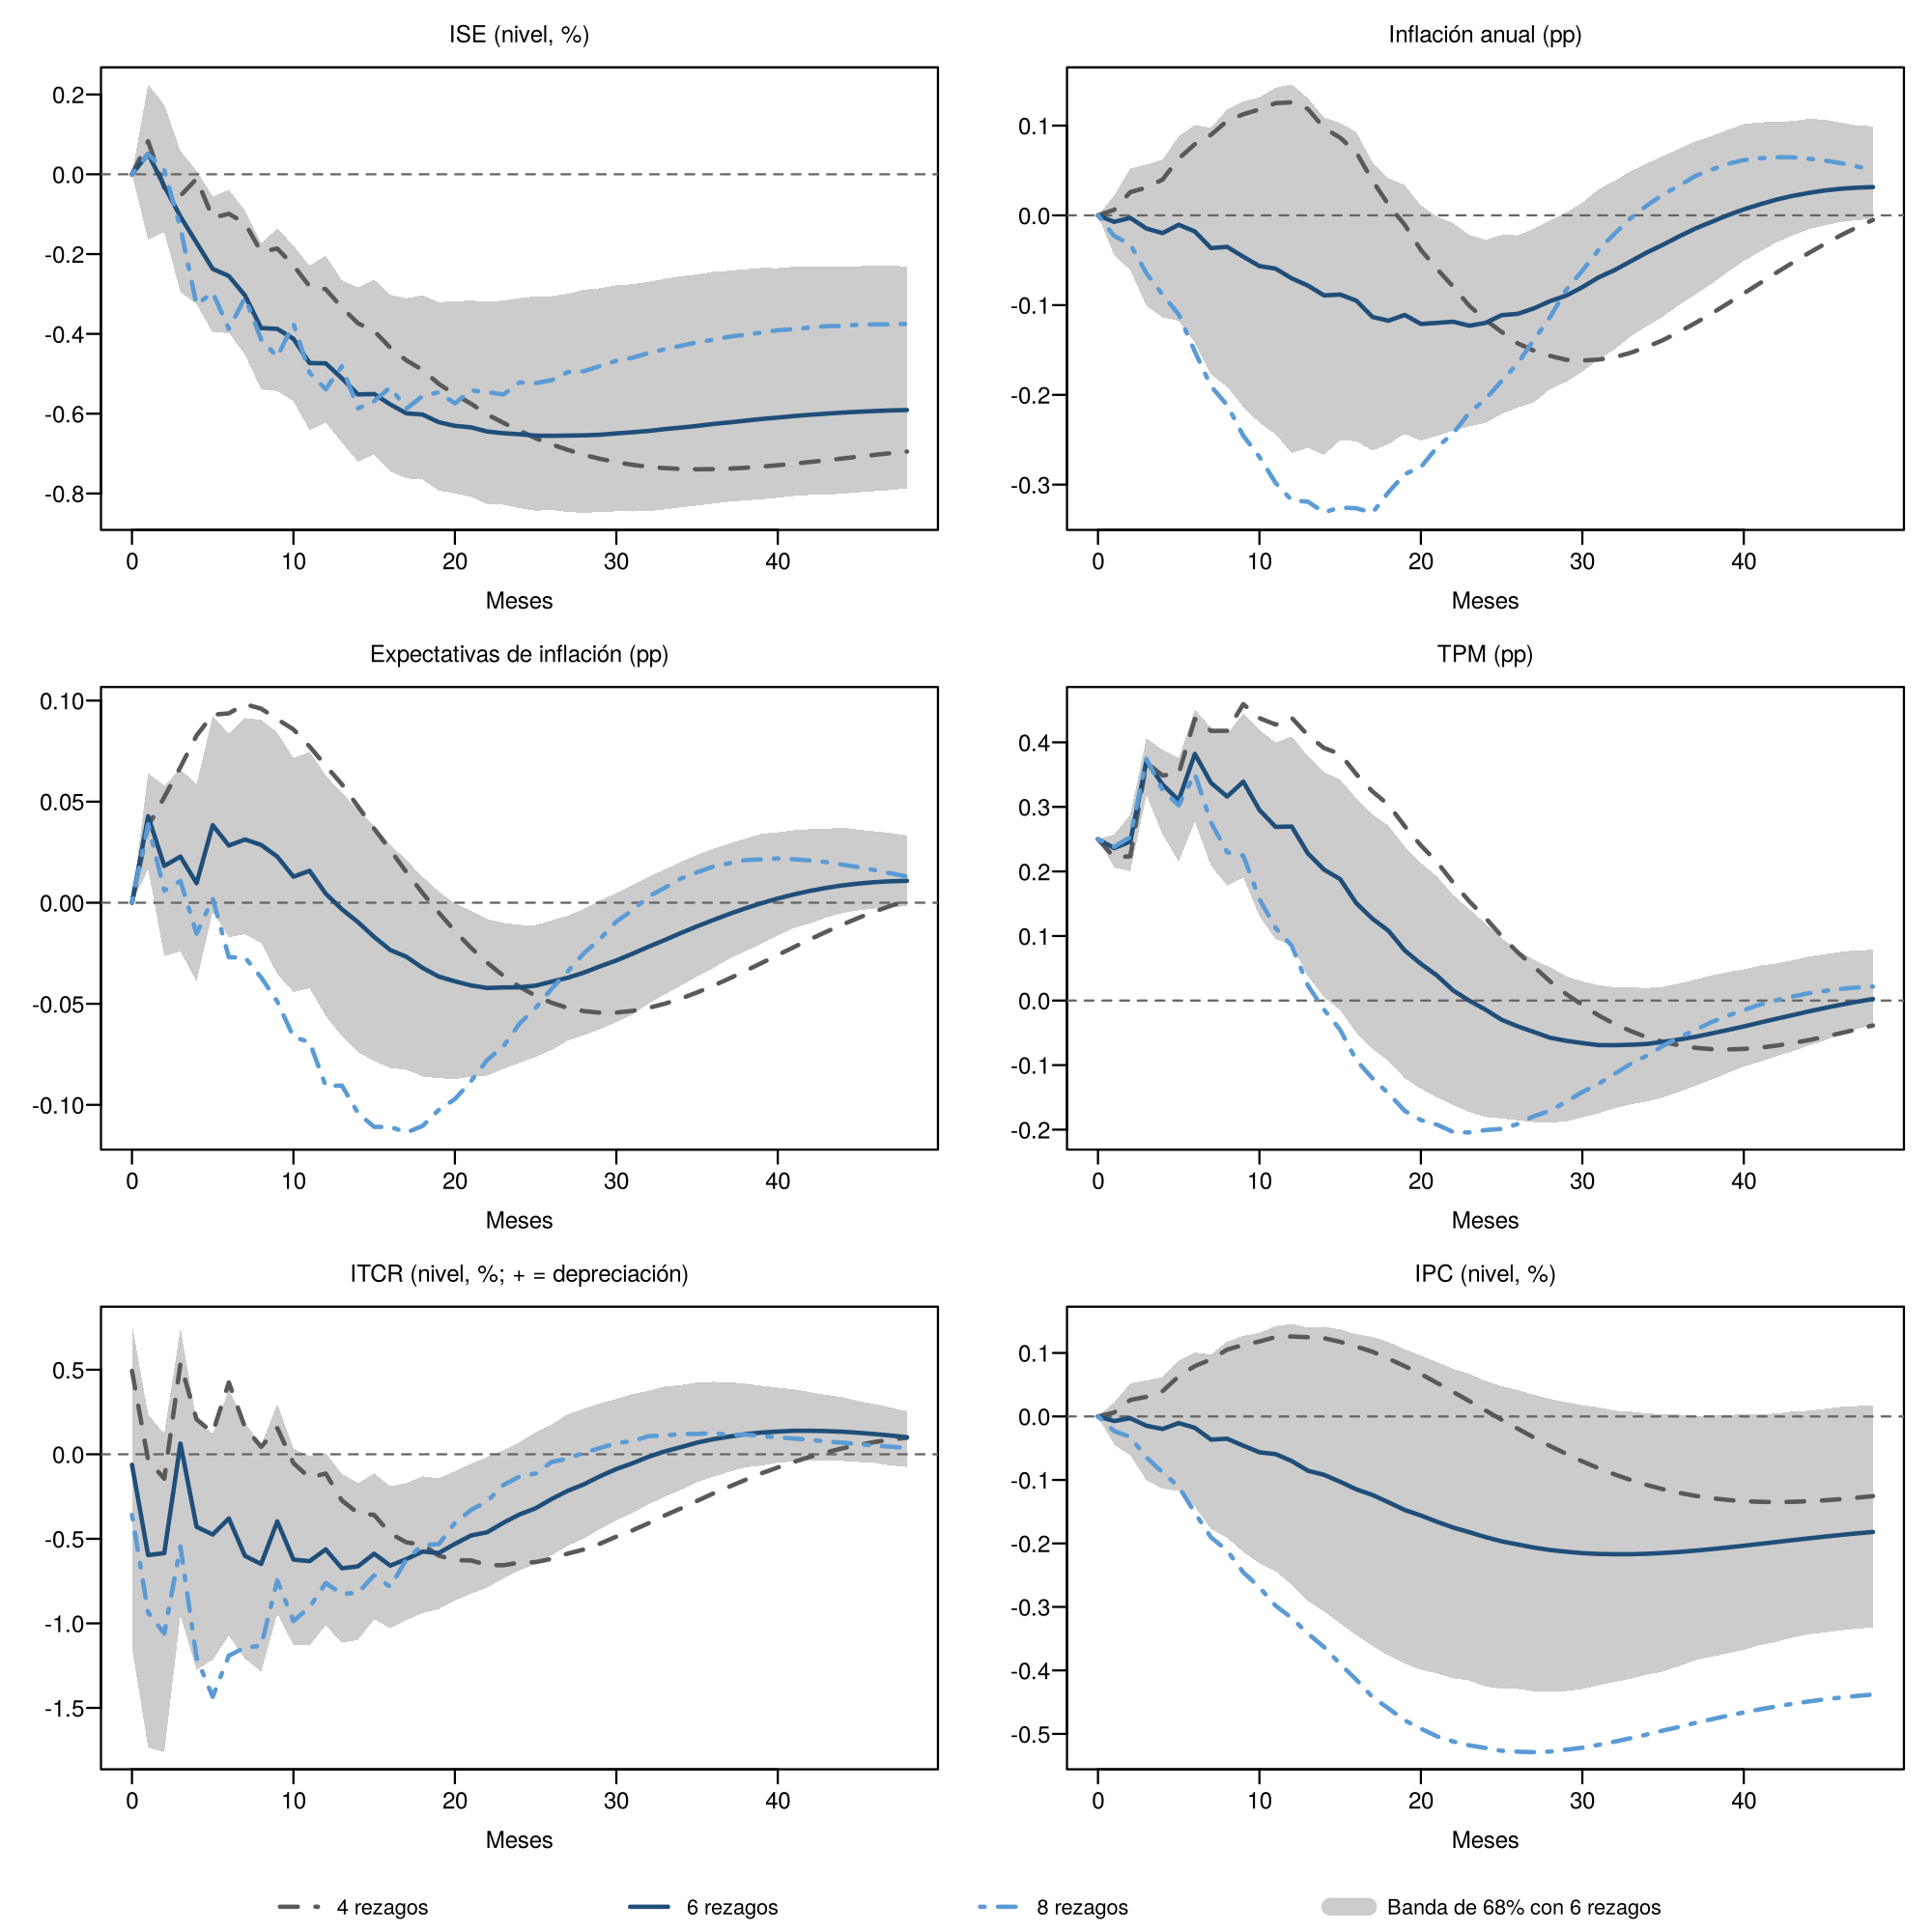
\includegraphics[width=0.85\textwidth]{irf_P1_rezagos_25pb.png}
\caption{Respuestas a un alza de 25 pb en la TPM con 4, 6 y 8 rezagos}
\label{fig:D_rezagos}
\notascuadro{\textit{Nota.} Banda del bootstrap por bloques de 12 meses (2,000 réplicas).

Fuente: Elaboración propia con datos de DANE y Banco de la República.}
\end{figure}

Ante estos resultados, podemos observar que la caída del ISE es robusta, y la eventual caída de la inflación y el ITCR, también. Sin embargo, los 4 rezagos no son recomendados por el AIC, y 8 tampoco es estadísticamente significativo.

Se reportan resultados:

\begin{itemize}
\item ITCR al impacto [banda de 68\%]: $+0.49$ [$-0.92$, $1.58$] (4 rezagos); $-0.06$ [$-1.14$, $0.77$] (6); $-0.36$ [$-1.65$, $0.78$] (8).
\item IPC, mes 24 [banda]: $+0.01$ [$-0.28$, $0.17$] (4); $-0.19$ [$-0.43$, $0.06$] (6); $-0.52$ [$-0.68$, $-0.05$] (8); con 8 rezagos y corrección, $-1.10$.
\item ISE, mes 24 [banda]: $-0.64$ [$-0.93$, $-0.37$] (4); $-0.65$ [$-0.84$, $-0.31$] (6); $-0.52$ [$-0.75$, $-0.17$] (8).
\end{itemize}


\paragraph{D.3.2 Sesgo de muestra pequeña y corrección de Kilian.}

\subparagraph{El sesgo.}

Kilian y Lütkepohl (2017) señalan que el estimador de mínimos cuadrados de los parámetros de pendiente puede estar sustancialmente sesgado en muestras pequeñas. Sin embargo, este sesgo puede ser estimado y corregido (Kilian, 1998). Es por esto que se lleva a cabo esta corrección, que si bien, no tiene fundamento teórico para cuando se presenta ARCH, se muestra como robustez.

En el siguiente cuadro se muestra, a través de la corrección, cómo es que cambia la persistencia de las variables, y el ángulo de la estimación.

\cuadro{cuadro_D_persistencia}

\subparagraph{Corrección con el algoritmo completo.}

% figura de prog/12_sesgo_completo_P1.R
\begin{figure}[H]
\centering
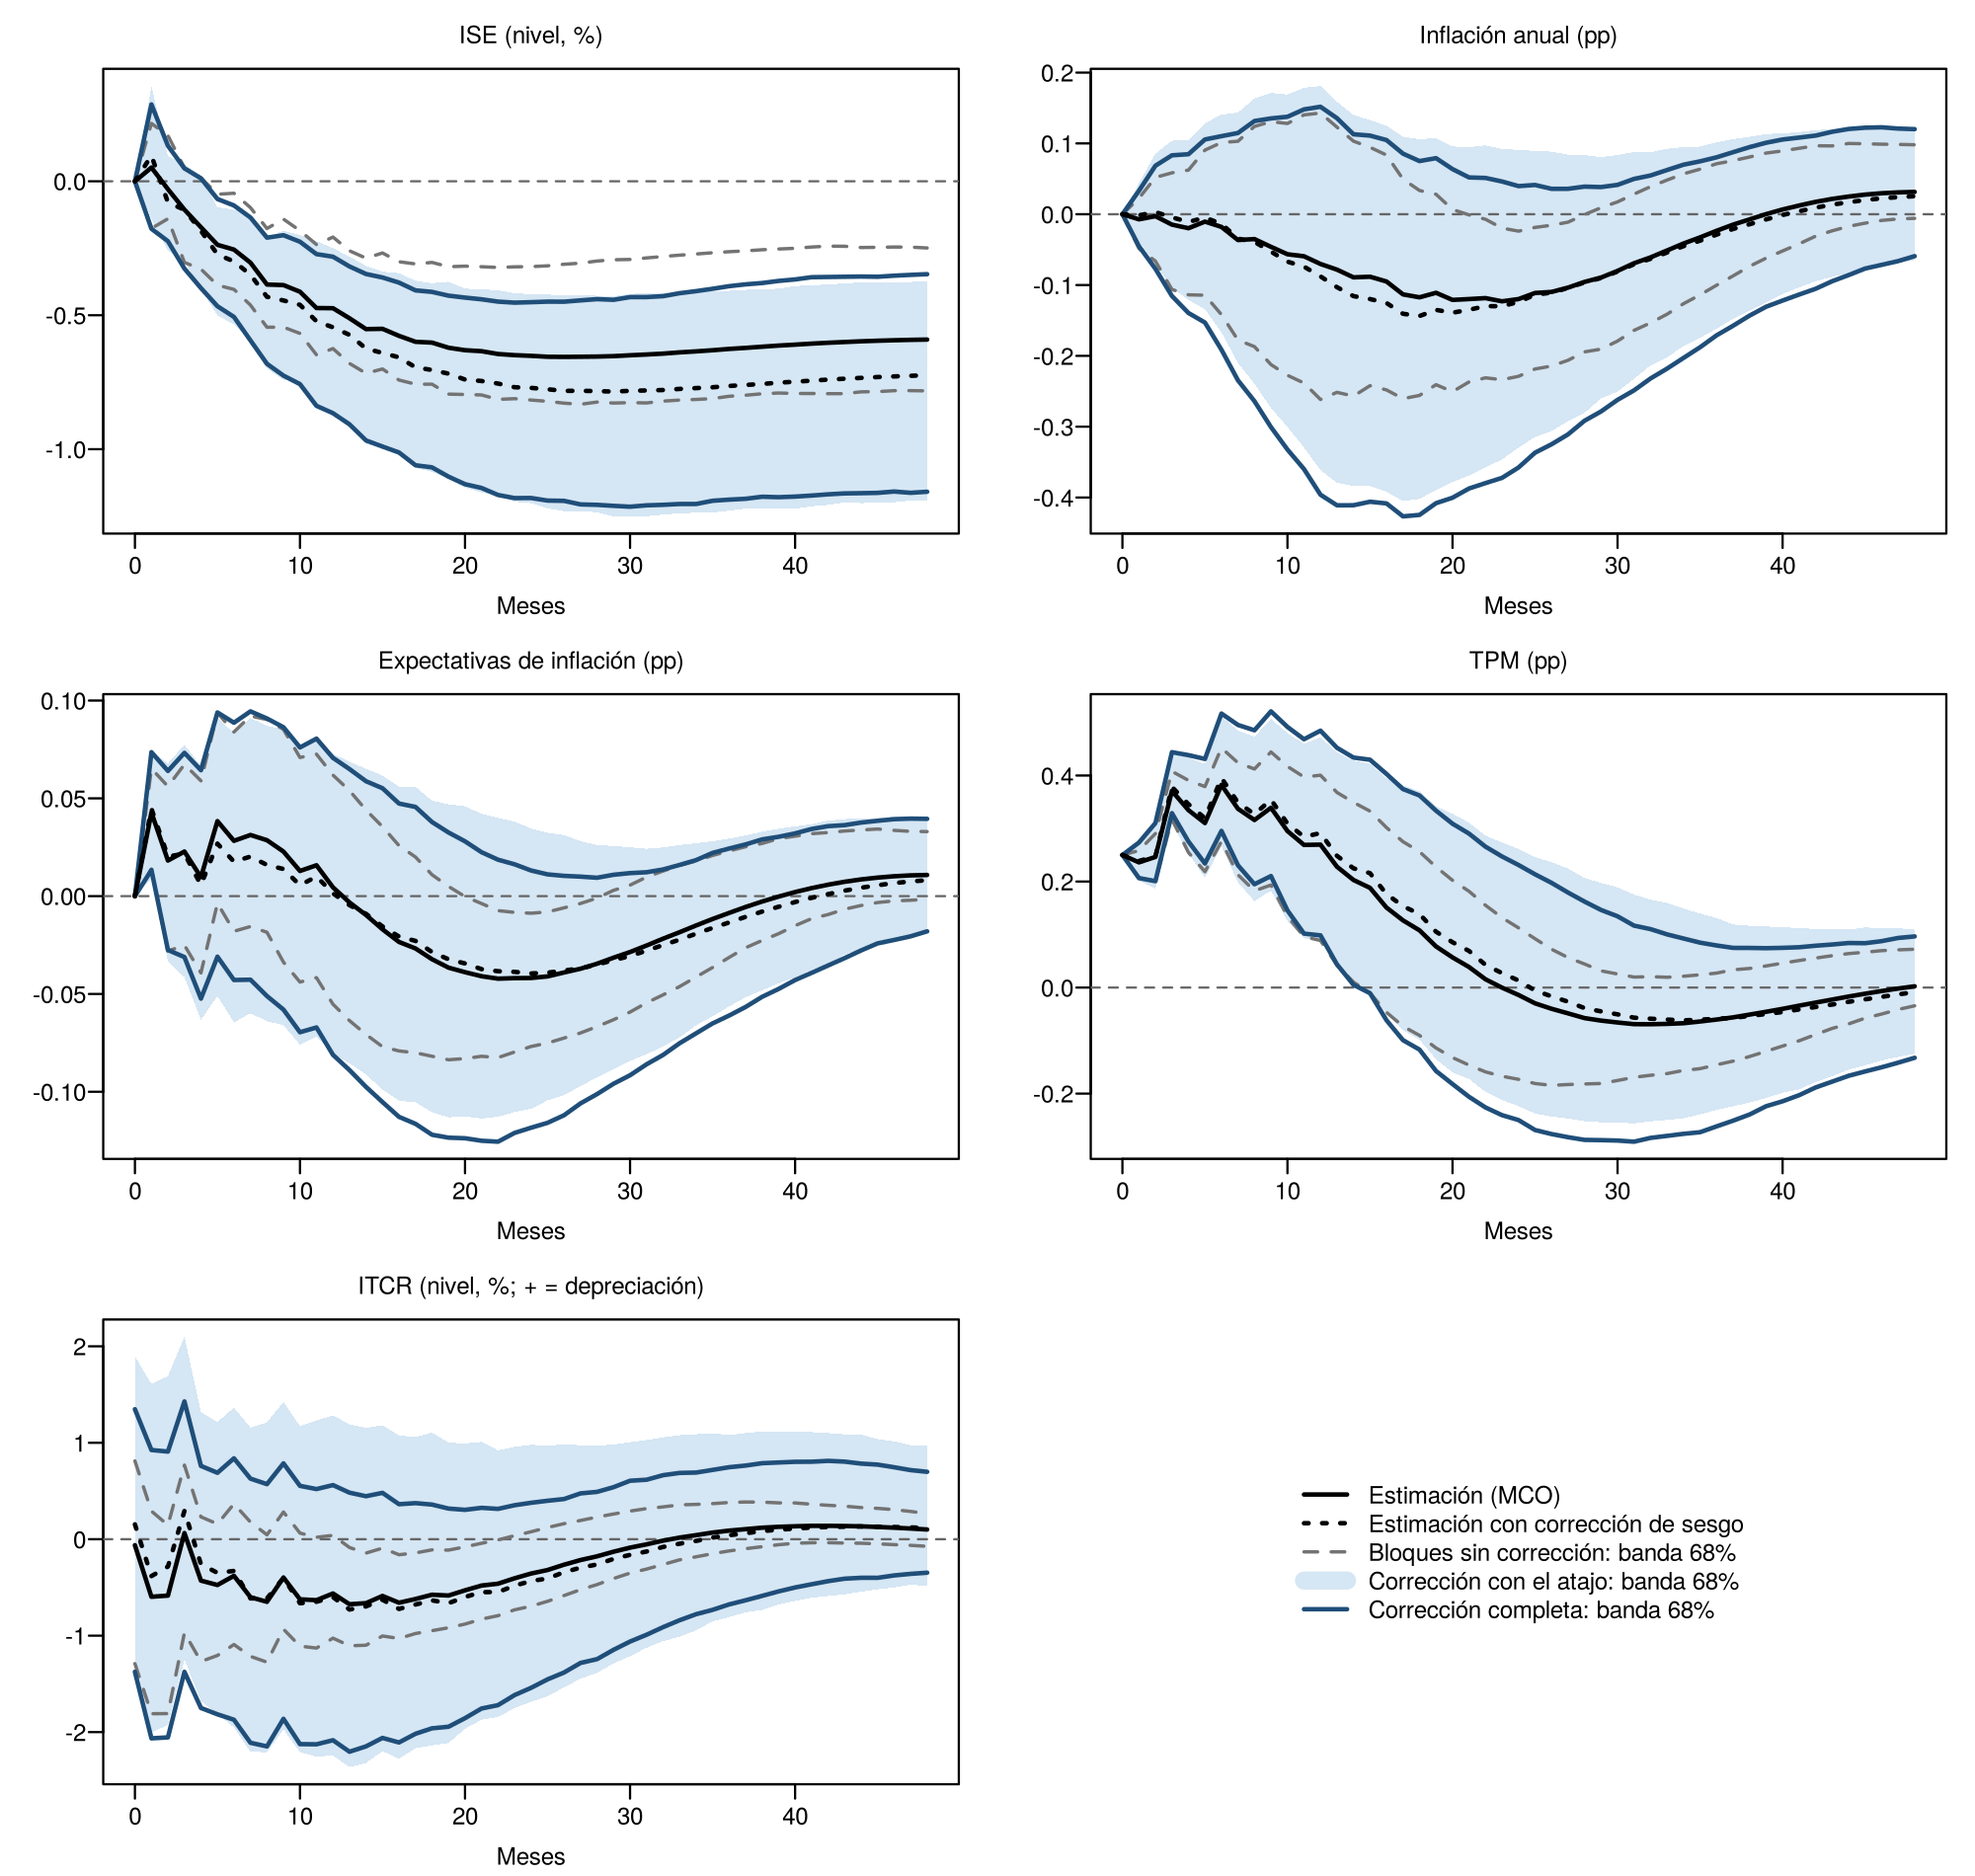
\includegraphics[width=0.85\textwidth]{irf_P1_sesgo_completo_25pb.png}
\caption{Bandas de 68\% sin corrección de sesgo, con el atajo y con la corrección completa}
\label{fig:D_sesgo_completo}
\notascuadro{\textit{Nota.} 2,000 réplicas por bloques de 12 meses; en la corrección completa, 500 réplicas anidadas por réplica.

Fuente: Elaboración propia con datos de DANE y Banco de la República.}
\end{figure}

Hay que notar, que ante la corrección de sesgo, la única caída que se mantiene significativa, es la del ISE.

Las bandas corregidas son más anchas, ya que algunas réplicas corregidas quedan cerca de una raíz unitaria y producen respuestas extremas.

De igual manera, es buen diagnóstico, que, como se observa en el Cuadro~\ref{tab:D_persistencia}, el ángulo corregido es muy similar al de MCO.

\cuadro{cuadro_D_sesgo_completo}

\paragraph{D.3.3 Otros métodos de inferencia: iid, \textit{wild} y Hall.}

En la Figura~\ref{fig:D_metodos} se observan los impulsos respuesta de cada variable, con las bandas construidas mediante distintos métodos. Se grafican las bandas por \textit{wild bootstrap}, por bloques de 12 meses según Hall (1992), y las conclusiones quedan similares.

% figura de prog/13_cuadros_anexo_D.R, con las bandas de prog/07_inferencia_P1.R
\begin{figure}[H]
\centering
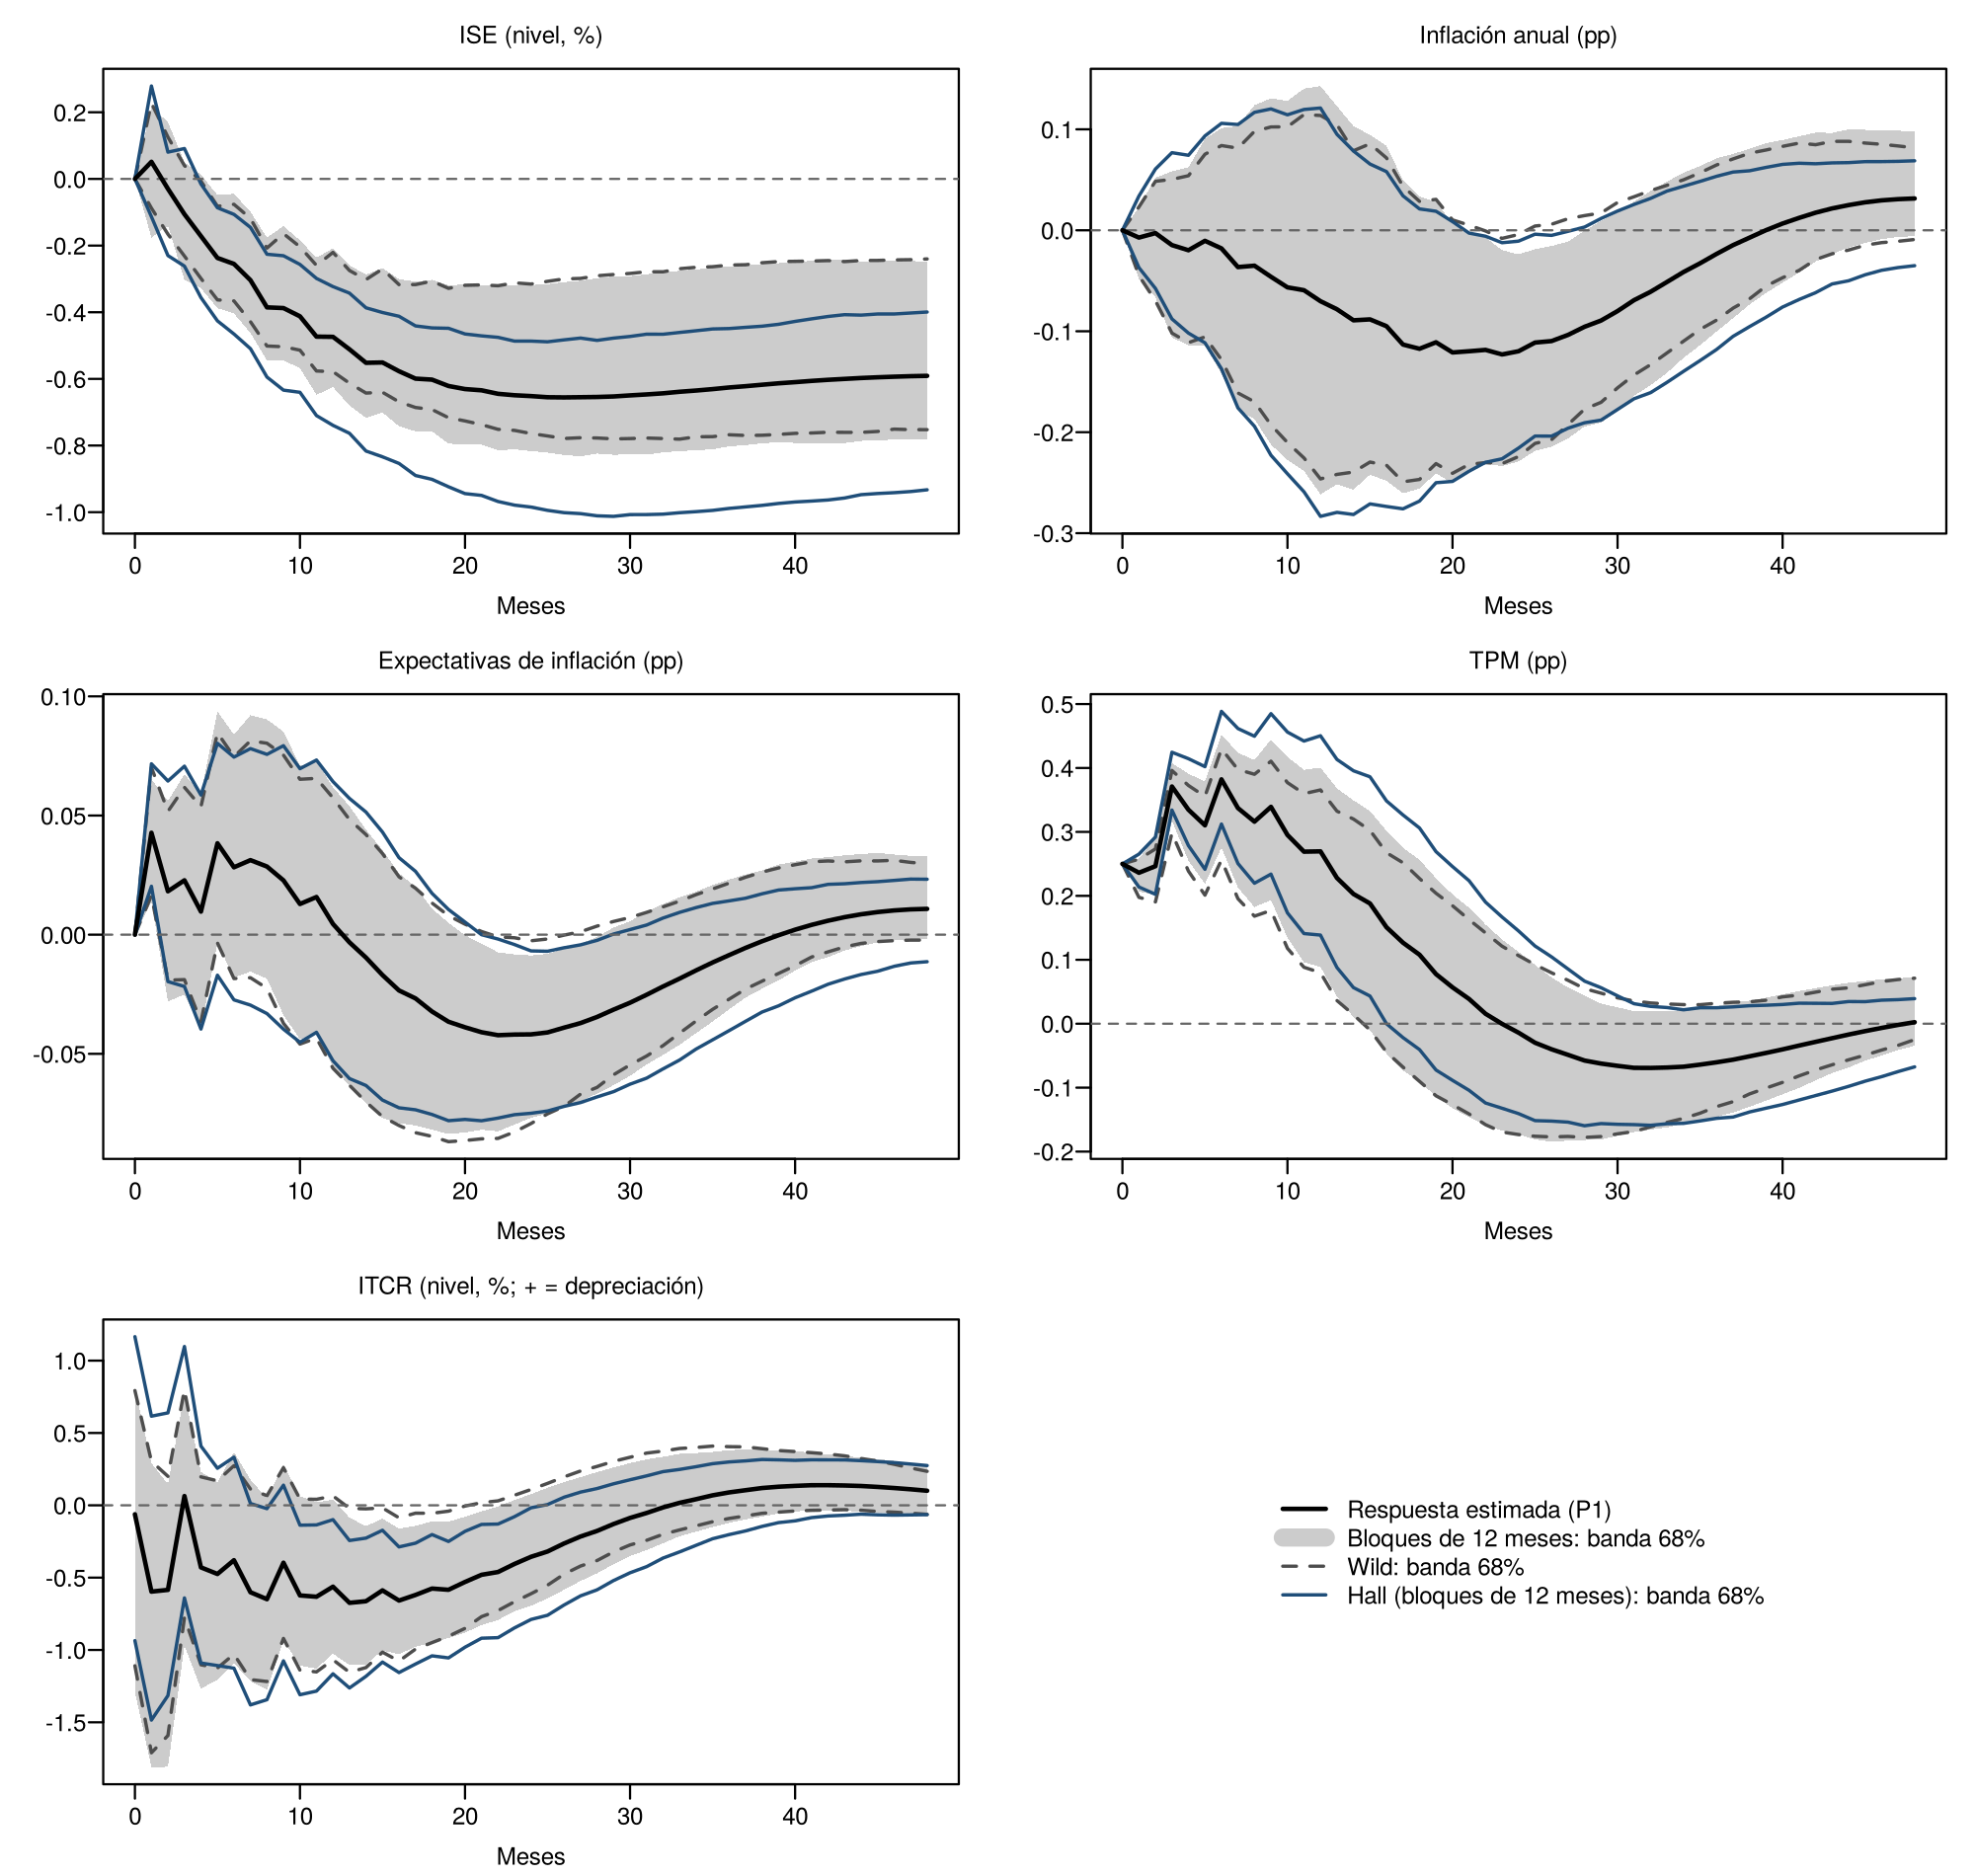
\includegraphics[width=0.85\textwidth]{irf_P1_metodos_25pb.png}
\caption{Bandas de 68\% con distintos métodos de inferencia: alza de 25 pb en la TPM}
\label{fig:D_metodos}
\notascuadro{\textit{Nota.} bloques de 12 meses y Hall: 2,000 réplicas; \textit{wild}: 1,000 réplicas.

Fuente: Elaboración propia con datos de DANE y Banco de la República.}
\end{figure}

Así mismo, en el Cuadro~\ref{tab:D_otros_metodos}, se presentan las bandas de 68\% con distintos métodos de inferencia.

\cuadro{cuadro_D_otros_metodos}

Esto muestra que, independientemente del método de inferencia, los resultados son similares a los de bloques de 12 meses. Por lo cual, los resultados se mantienen robustos ante distintos métodos de inferencia.

\paragraph{D.3.4 Especificaciones 9 y 10.}

% Identificación de las especificaciones 9 y 10, con base en Identificacion_P8_P9.pdf (prog/05_propuestas_P8_P9.R y
% prog/06_propuesta_P10.R). Se sortean 2,000 formas reducidas de la posterior y 40 ángulos uniformes en
% (-pi/2, pi/2) por sorteo; se conservan los que cumplen las restricciones.
\subparagraph{Identificación de la especificación 9.}

Por último, para mayor robustez, se presenta la estimación del mismo choque con distinta identificación.

Primero, se presenta, con la misma forma reducida, una identificación mediante restricciones de corto plazo y restricciones de signos (Uhlig, 2005; Arias, Rubio-Ramírez y Waggoner, 2018).

Se impone un signo positivo en la ecuación de la TPM para los primeros seis periodos, un signo negativo para el ITCR en los primeros seis periodos, además de que se conservan los nueve ceros, de la especificación inicial.

Además, se añade una cota sobre la reacción del ITCR sobre la TPM.
\begin{equation}\label{eq:D_H}
H = \begin{pmatrix}
h_{11} & 0 & 0 & 0 & 0\\
h_{21} & h_{22} & 0 & 0 & 0\\
h_{31} & h_{32} & h_{33} & 0 & 0\\
h_{41} & h_{42} & h_{43} & \boxed{\,{+}\,} & h_{45}\\
h_{51} & h_{52} & h_{53} & \boxed{\,{-}\,} & h_{55}
\end{pmatrix},
\qquad h_{54} \ge -\kappa\, h_{44}, \quad \kappa = 10.
\end{equation}
Los signos están justificados por la teoría previa que se ha comentado, y se fija $\kappa = 10$ como una cota holgada (Kilian y Murphy, 2012). Según González-Téllez y Laborde-Vera (2026), con los choques de Bloomberg, el peso se aprecia cerca de 6\% en el impacto y 8\% un periodo después, por lo cual funciona como cota holgada.

Los signos se mantienen en los meses 1 a 5.
\begin{equation}\label{eq:D_signos}
\underbrace{\begin{pmatrix} \mathrm{ISE}_0\\ \pi_0\\ \pi^e_0\\ i_0\\ q_0 \end{pmatrix} =
\begin{pmatrix} 0\\ 0\\ 0\\ {>}\,0\\ {\le}\,0 \end{pmatrix}}_{\text{impacto, } h=0},
\qquad
\underbrace{\begin{pmatrix} \mathrm{ISE}_h\\ \pi_h\\ \pi^e_h\\ i_h\\ q_h \end{pmatrix} =
\begin{pmatrix} *\\ *\\ *\\ {\ge}\,0\\ {\le}\,0 \end{pmatrix}}_{h = 1,\dots,5},
\qquad q_0 \in [-\kappa\, i_0,\ 0].
\end{equation}

Se calcula $H$, se obtiene el factor de Cholesky $P$ y por la rotación de Givens en el plano de los choques 4 y 5:
\begin{equation}\label{eq:D_rotacion}
H(\theta) = P\,Q(\theta), \qquad
Q(\theta) = \begin{pmatrix} I_3 & 0\\ 0 & R(\theta) \end{pmatrix}, \qquad
R(\theta) = \begin{pmatrix} \cos\theta & -\sin\theta\\ \sin\theta & \cos\theta \end{pmatrix},
\end{equation}
\begin{equation}\label{eq:D_h4}
h_4(\theta) = \cos\theta\, P_{\cdot 4} + \sin\theta\, P_{\cdot 5} = \bigl(0,\ 0,\ 0,\ P_{44}\cos\theta,\ P_{54}\cos\theta + P_{55}\sin\theta\bigr)'.
\end{equation}
Se sortea $\theta$ y se conservan los ángulos que corresponden a las restricciones.

La cota puede ser vista como elasticidad de impacto, como es una función invertible, fijar la cota, equivale a fijar un ángulo:
\begin{equation}\label{eq:D_eta}
\eta(\theta) \equiv \frac{h_{54}}{h_{44}} = \frac{P_{54} + P_{55}\tan\theta}{P_{44}} \qquad (\%\ \text{por pp}),
\end{equation}
\begin{equation}\label{eq:D_thmin}
\eta(\theta) \ge -\kappa \iff \theta \ \ge\ \theta_{\min}(\kappa) = \arctan\!\left(-\frac{\kappa P_{44} + P_{54}}{P_{55}}\right).
\end{equation}

\subparagraph{Identificación de la especificación 10.}

Para mayor robustez, se fija otra especificación, en donde la identificación es la misma que en el ejercicio anterior, pero cambian las variables y la forma reducida. Entran las variables en niveles, y se toman 12 rezagos.
\begin{equation}\label{eq:D_var10}
y_t = (100\ln \mathrm{ISE}_t,\ 100\ln \mathrm{IPC}_t,\ \pi^e_t,\ i_t,\ 100\ln \mathrm{TRM}_t)', \qquad
y_t = c + \sum_{j=1}^{12} A_j y_{t-j} + \Gamma x_t + u_t,
\end{equation}
\begin{equation}\label{eq:D_signos10}
\underbrace{\begin{pmatrix} \mathrm{ISE}_0\\ \mathrm{IPC}_0\\ \pi^e_0\\ i_0\\ s_0 \end{pmatrix} =
\begin{pmatrix} 0\\ 0\\ 0\\ {>}\,0\\ {\le}\,0 \end{pmatrix}}_{\text{impacto, } h=0},
\qquad
\underbrace{\begin{pmatrix} \mathrm{ISE}_h\\ \mathrm{IPC}_h\\ \pi^e_h\\ i_h\\ s_h \end{pmatrix} =
\begin{pmatrix} *\\ *\\ *\\ {\ge}\,0\\ {\le}\,0 \end{pmatrix}}_{h = 1,\dots,5},
\qquad s_0 \in [-\kappa\, i_0,\ 0].
\end{equation}
Las variables están en niveles, entonces $s_h$, la TRM nominal, no se acumula.

Se realiza inferencia bayesiana para estos ejercicios de robustez.

En la Figura~\ref{fig:D_P9} se grafican las respuestas puntuales de la identificación principal del trabajo, y la propuesta con restricciones de signos (manteniendo la forma reducida).
En la Figura~\ref{fig:D_P10} se grafican las dos identificaciones mediante signos, P10 corresponde a la forma reducida con 12 rezagos y con variables en niveles.

% figura de prog/05_propuestas_P8_P9.R
\begin{figure}[H]
\centering
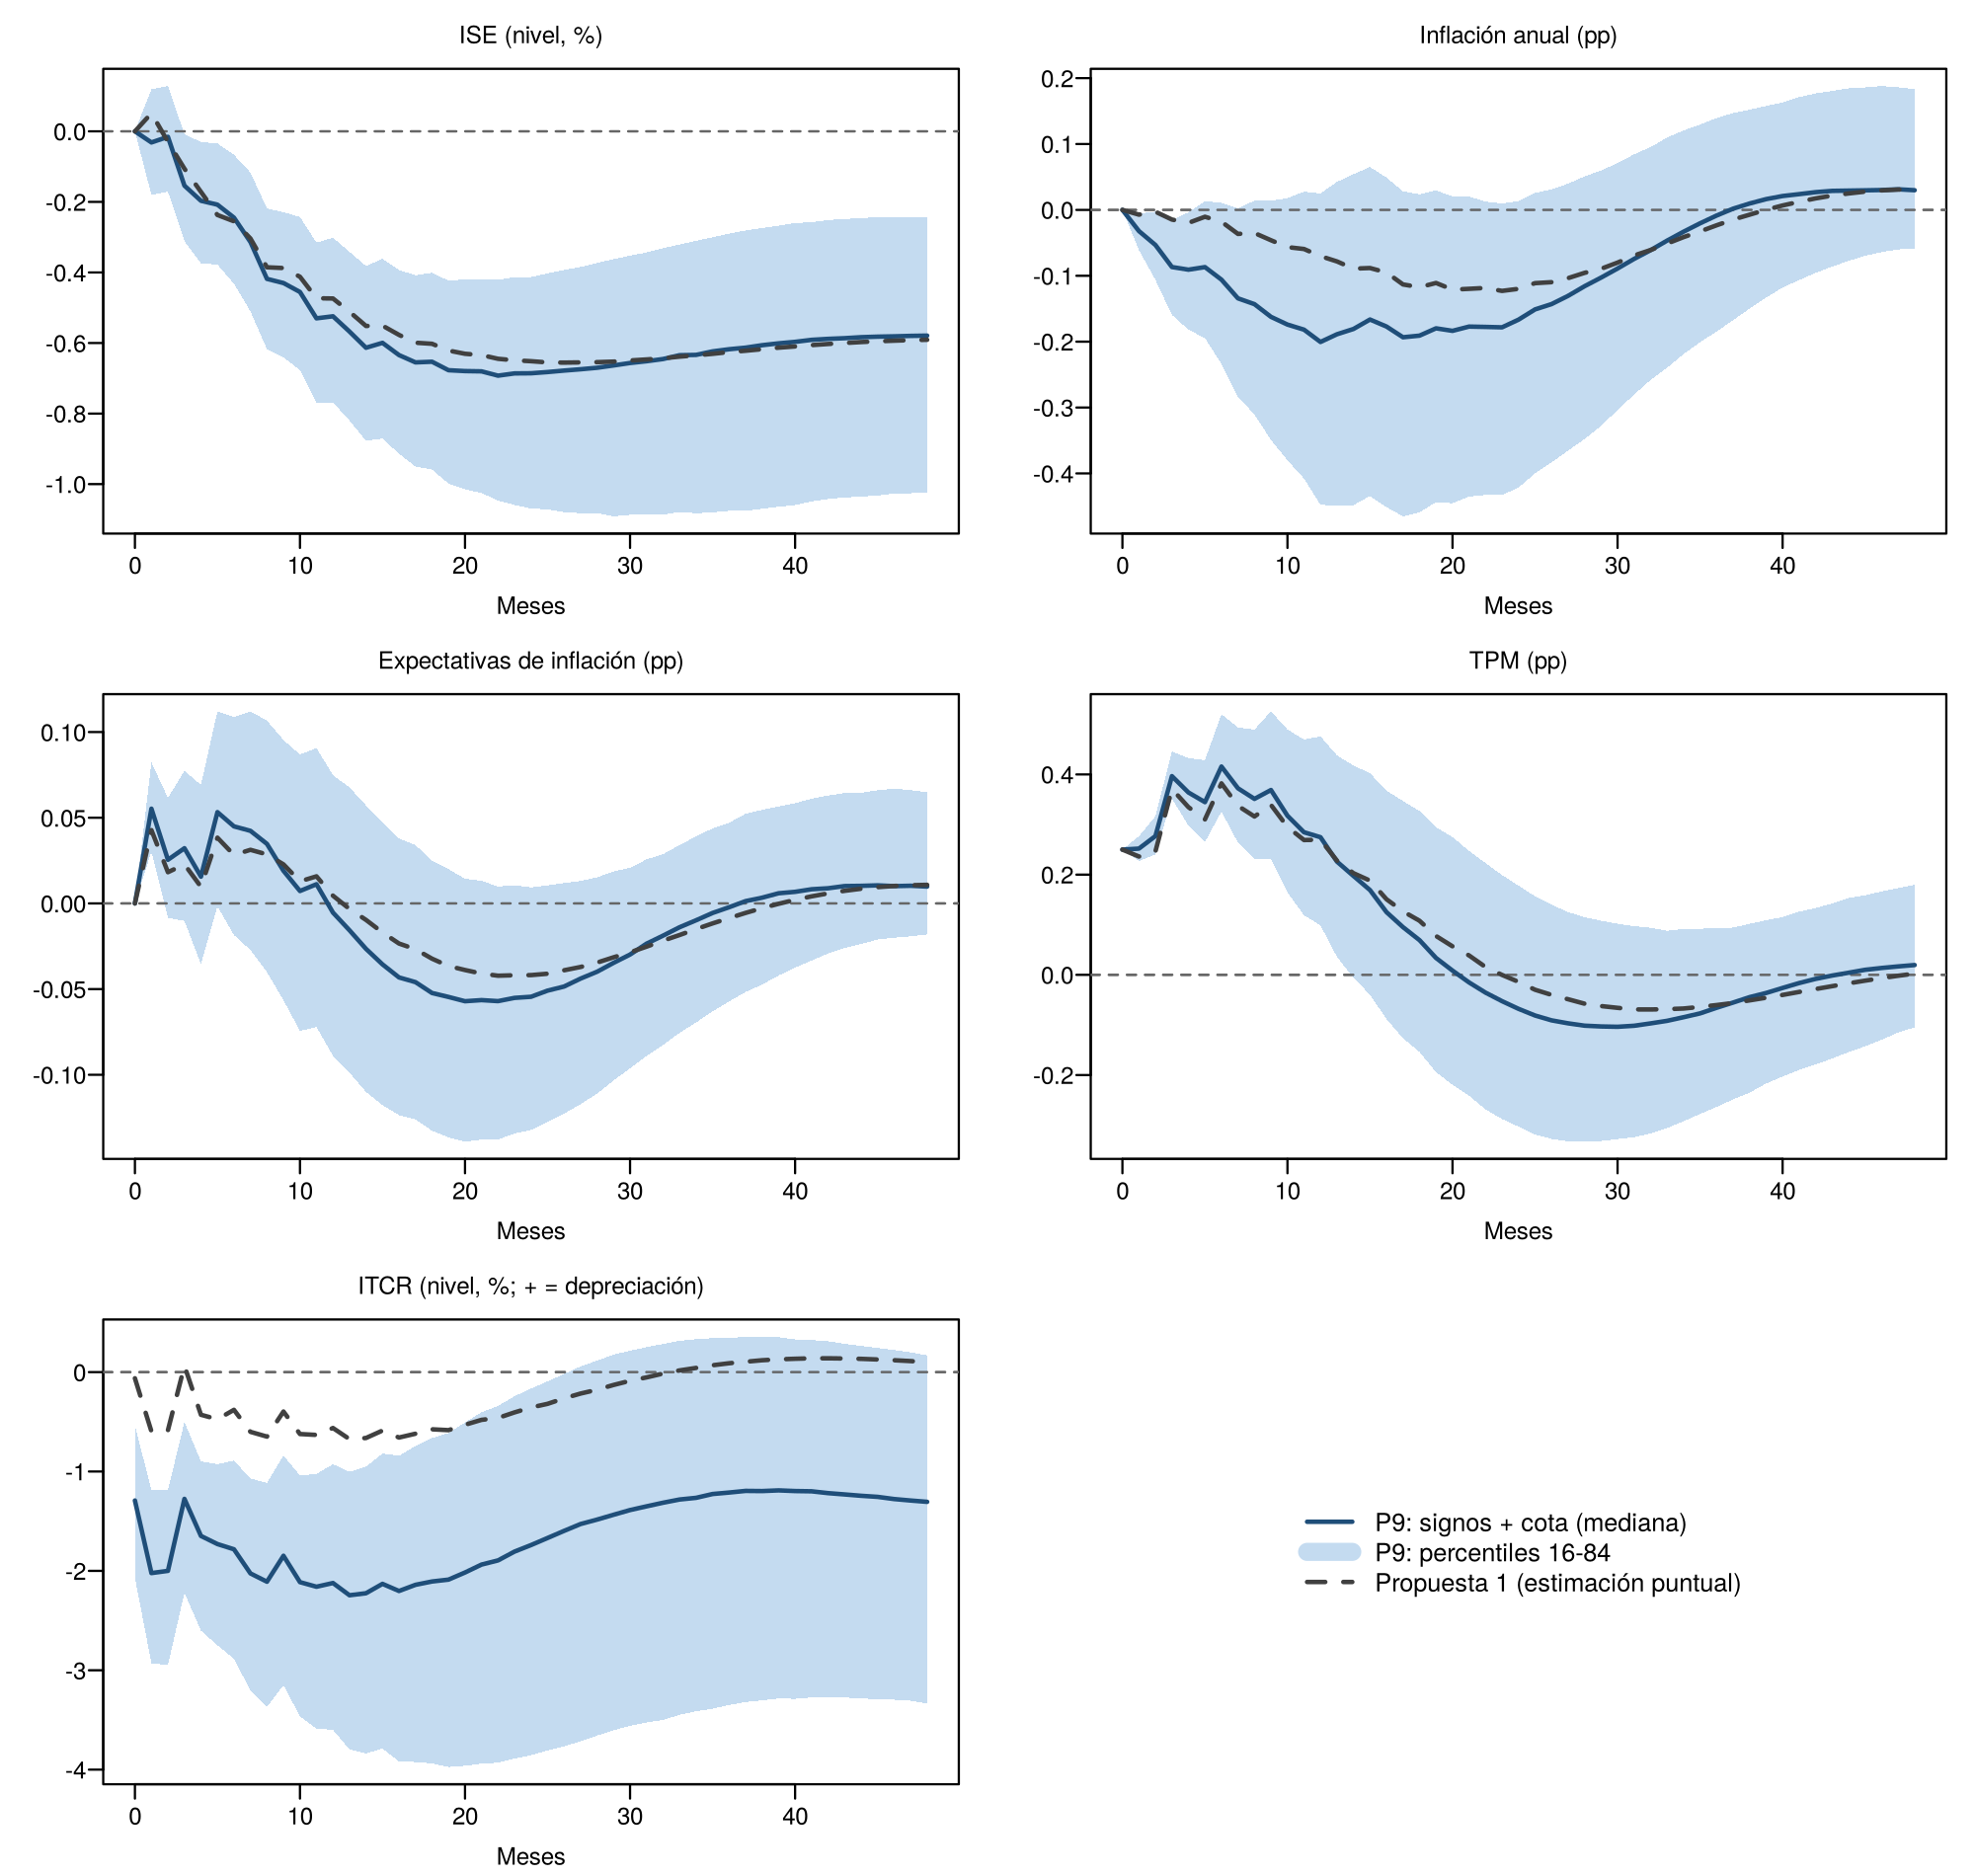
\includegraphics[width=0.85\textwidth]{irf_P9_vs_P1_25pb.png}
\caption{Especificación 9 frente a la especificación 1: alza de 25 pb en la TPM}
\label{fig:D_P9}
\notascuadro{\textit{Nota.} Especificación 9: 14,782 modelos aceptados de 80,000 (2,000 sorteos de la forma reducida por 40 rotaciones).

Fuente: Elaboración propia con datos de DANE y Banco de la República.}
\end{figure}

% figura de prog/06_propuesta_P10.R
\begin{figure}[H]
\centering
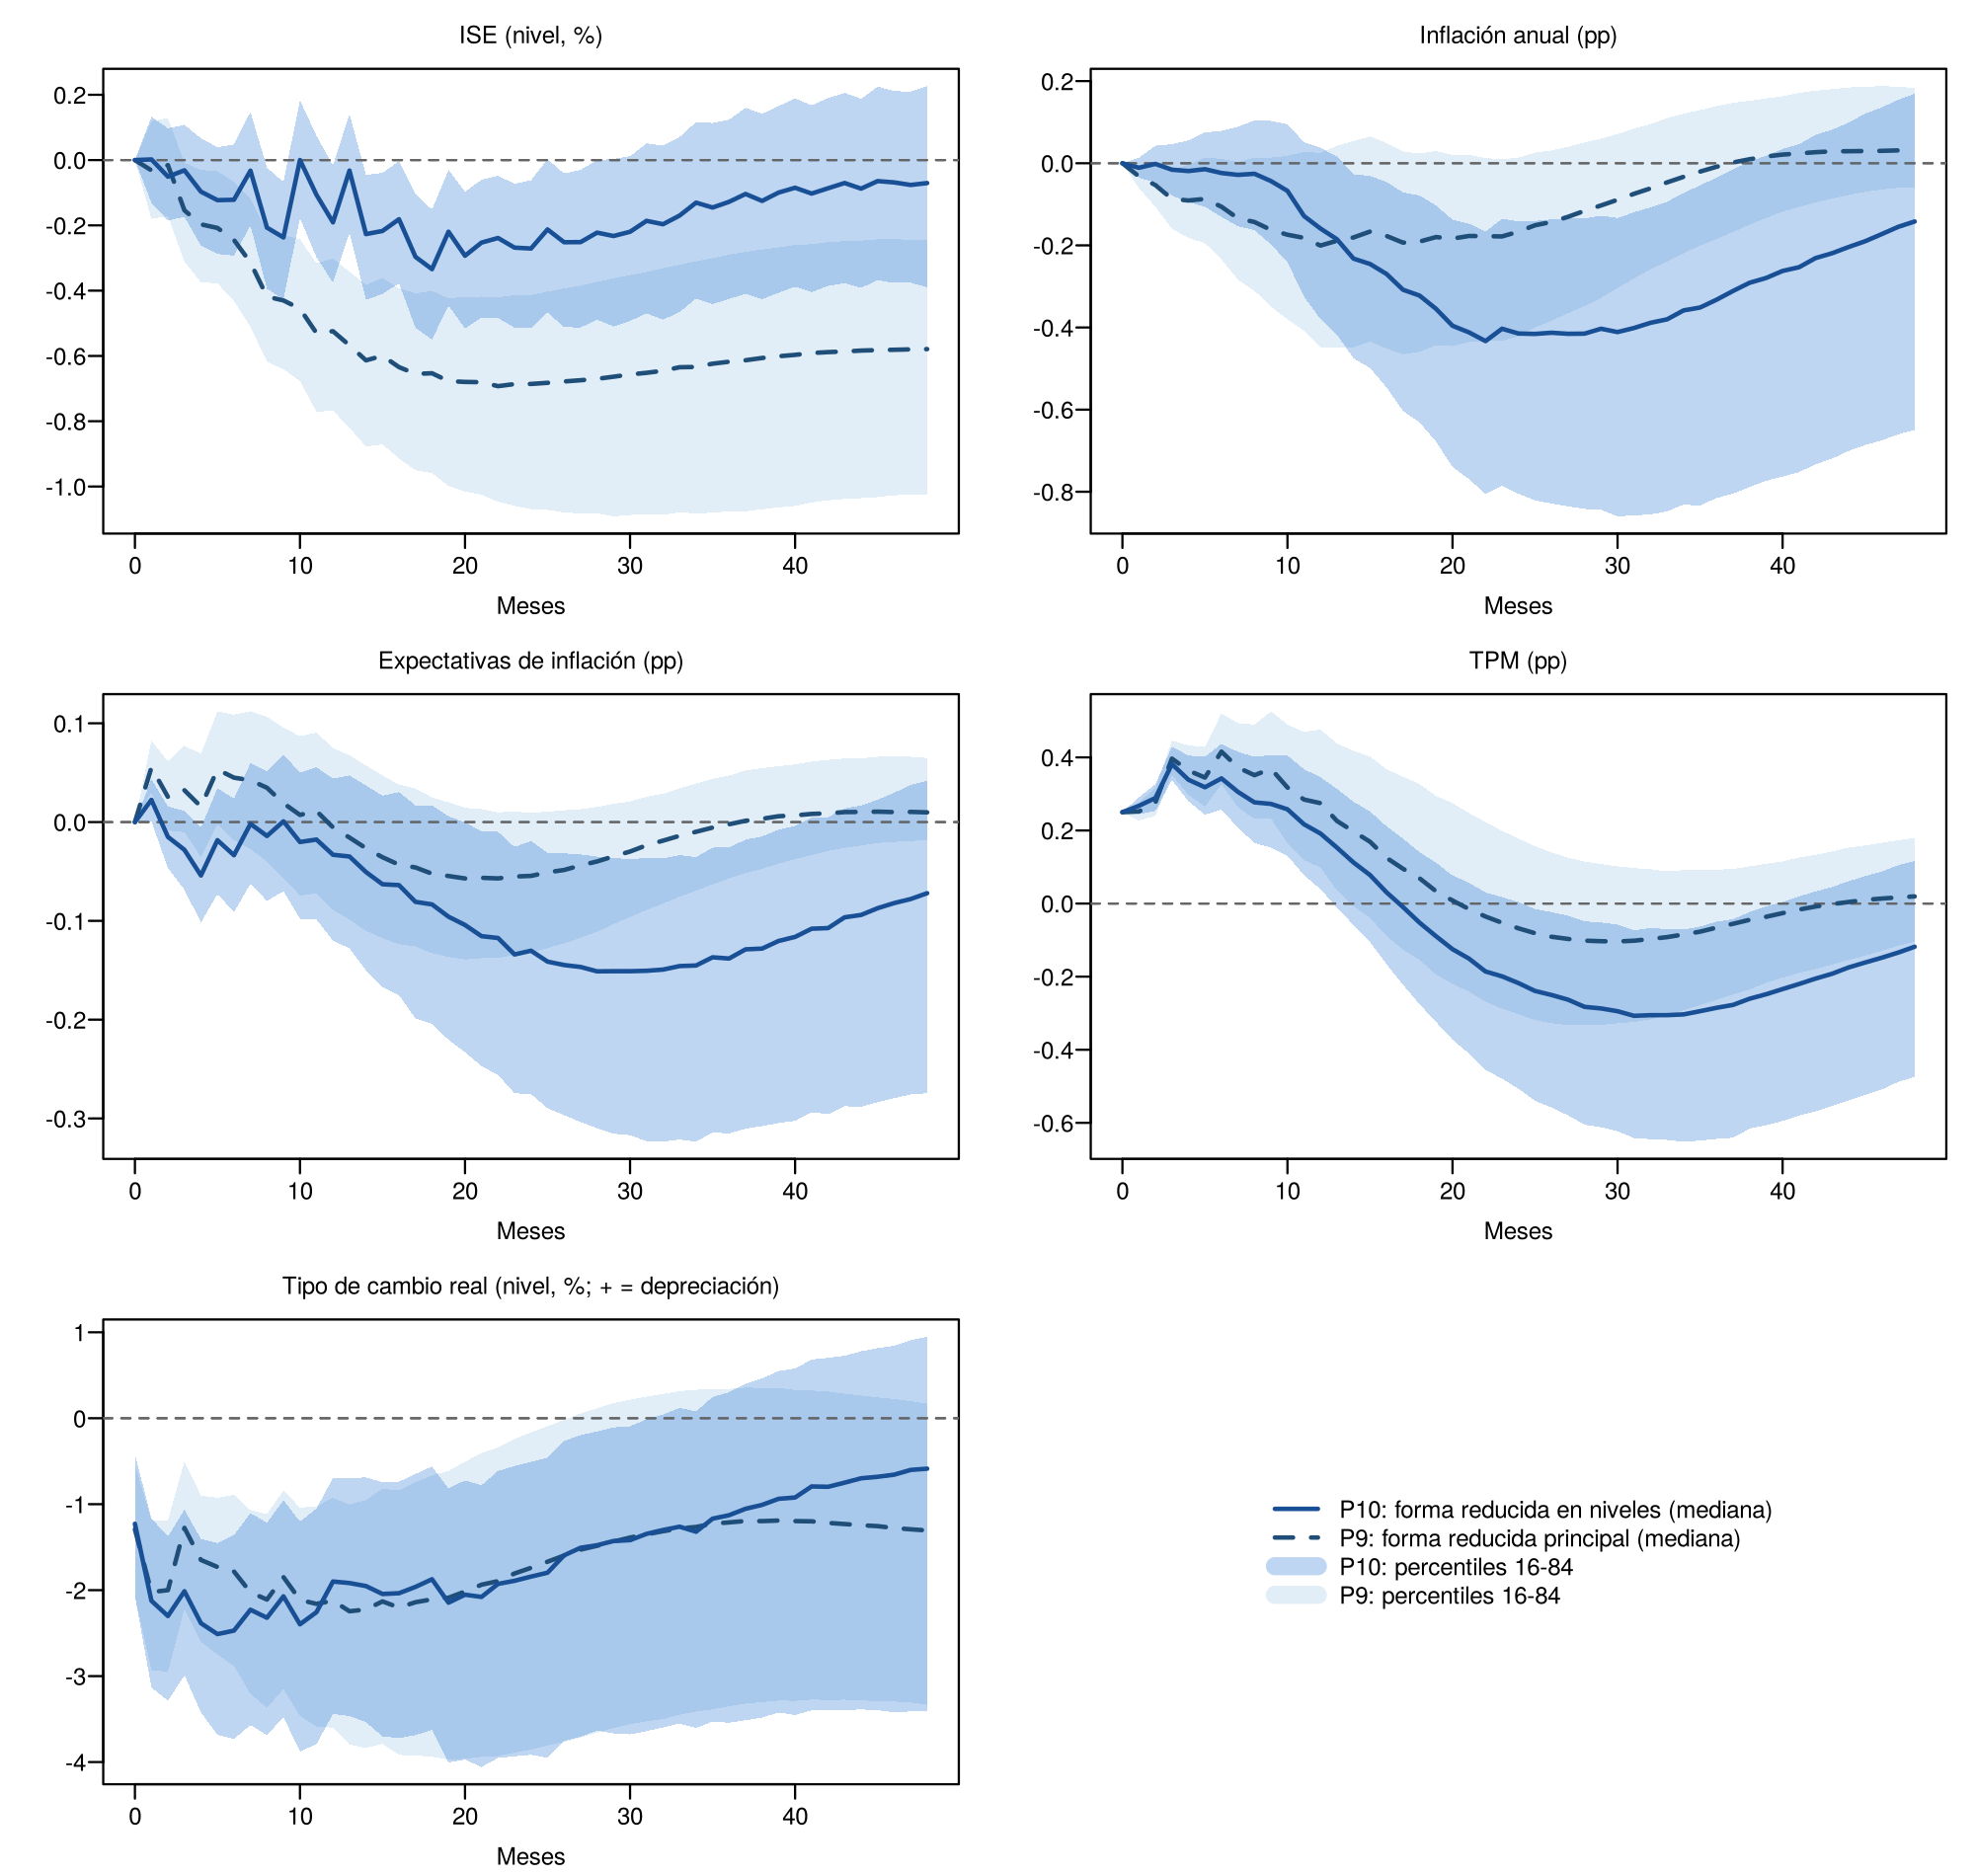
\includegraphics[width=0.85\textwidth]{irf_P10_vs_P9_25pb.png}
\caption{Especificación 10 frente a la especificación 9: alza de 25 pb en la TPM}
\label{fig:D_P10}
\notascuadro{\textit{Nota.} Especificación 10: forma reducida en niveles, 12 rezagos, 2006m1--2026m7.

Fuente: Elaboración propia con datos de DANE y Banco de la República.}
\end{figure}

En las Figuras~\ref{fig:D_P9} y~\ref{fig:D_P10} se puede notar que las respuestas ante el choque de política monetaria, son similares entre especificaciones.

No hay diferencias sustanciales entre estos métodos de identificación, y la propuesta original. Por lo cual, los resultados son robustos ante distintas especificaciones.

% =============================================================================
\subsubsection*{D.4 Conclusiones}

Dadas las distintas pruebas de robustez, con distintos rezagos, métodos de inferencia e identificación, se llega a la conclusión de que:

\begin{enumerate}[label=\arabic*), leftmargin=2em, itemsep=2pt, topsep=4pt]
\item La caída del ISE ante el alza de 25 pb en la TPM, es estadísticamente significativa, ante cualquier especificación y prueba de robustez.
\item La inflación anual, cae significativamente en distintas especificaciones, aunque al corregir por sesgo, no se observa una caída estadísticamente significativa.
\item El ITCR, cae con significancia estadística en diversas especificaciones, pero tampoco sobrevive a la corrección de sesgo.
\item Las expectativas de inflación suben en el primer mes, y a partir de ahí caen hasta alcanzar un mínimo en el mes 22--23, siendo estadísticamente significativa esa caída. Ante correcciones de sesgo, tampoco sobrevive.
\end{enumerate}

De modo que, las respuestas ante el choque de política monetaria tienen sentido económico, pierden significancia, salvo la del ISE, solo ante corrección de sesgo, aunque este no está justificado cuando se presenta ARCH, como es el caso de este ejercicio. Sin embargo, se muestra por robustez.

\end{document}